\documentclass[journal,twocolumn]{IEEEtran}

\usepackage{amsmath,amssymb,amsfonts,amsthm}
\usepackage{booktabs,tabularx,multirow,makecell,array}
\usepackage{graphicx,xcolor}
\usepackage{cite}
\usepackage{microtype}
\usepackage{url}
\usepackage{bm}
\usepackage{adjustbox}
\usepackage{hyperref}

\hypersetup{
    colorlinks=true,
    linkcolor=blue!80!black,
    citecolor=blue!80!black,
    urlcolor=blue!80!black
}

\newtheorem{theorem}{Theorem}
\newtheorem{lemma}{Lemma}

\graphicspath{{figures/}}

\begin{document}

\title{Deconstructing Quantum Advantage and Data Leakage in Clinical Machine Learning: A Multi-Dataset Cross-Methodology Audit on Diabetes Benchmarks}

\author{Autonomous~Academic~Audit~Group
\thanks{Manuscript submitted to IEEE Transactions on Neural Networks and Learning Systems. The authors are with the Department of Biomedical Informatics and Computational Intelligence. Correspondence: research.audit@academic-audit.org.}
}

\markboth{IEEE Transactions on Neural Networks and Learning Systems,~Vol.~XX, No.~XX,~2026}%
{Autonomous Academic Audit Group: Deconstructing Quantum Advantage and Data Leakage in Clinical Machine Learning}

\maketitle

\begin{abstract}
Recent literature in quantum machine learning (QML) and healthcare artificial intelligence has reported near-perfect diagnostic accuracies ($94\%$ to $>99\%$) and claimed empirical quantum advantage on clinical diabetes benchmarks. In this work, we present an independent, multi-dataset, cross-methodology audit examining eight prominent published architectures across four distinct clinical diabetes cohorts: Pima Indians Diabetes ($N=768$, $d=8$), Sylhet Early-Stage Diabetes ($N=520$, $d=16$), a CDC BRFSS epidemiological extract ($N=2{,}000$, $d=21$), and the UCI 130-US Hospitals inpatient readmission database ($N=2{,}000$, $d=47$). 

Through rigorous cryptographic and algorithmic deconstruction, we reveal that published high-performance claims are artifacts of pervasive methodological flaws rather than genuine quantum superiority. Specifically: (1) \textbf{The Data Leakage Collapse}: in the Sylhet questionnaire cohort, 376 of 520 records belong to identical duplicate response clusters (comprising only 251 unique patient profiles); naive random train/test splits inadvertently place identical feature vectors in both partitions, inflating accuracy. When evaluated under strict group-aware cross-validation (\texttt{StratifiedGroupKFold}), model performance collapses by up to $22.1\%$ (e.g., Yadav ZZ-QSVM drops from $94.2\%$ to $72.1\%$, Daga ZZ-QSVM drops from $93.3\%$ to $73.3\%$, and classical Random Forest drops from $98.1\%$ to $93.0\%$). (2) \textbf{Published Mathematical and Methodological Anomalies}: we prove that Kotha et al.'s reported $\text{ROC-AUC}=1.00$ on 150 test instances containing 25 classification errors directly violates the Mann-Whitney $U$ upper bound ($\text{AUC}_{\max} \le 0.9700$); Kiran et al.'s headline $99.7\%$ accuracy is contradicted by their own reported $4\%$ error rate ($0.960$); Young's high F1 scores stem from global Gaussian Mixture Model oversampling that artificially inflates disease prevalence from $34.9\%$ to $81.9\%$; and Daga et al.'s global Gram matrix pre-computation introduces optimistic feature leakage. (3) \textbf{Statistical Parity and Absence of Quantum Advantage}: across 15 clean resampled folds, Nadeau-Bengio corrected paired $t$-tests with Holm step-down multiple-testing control establish that no pure quantum kernel (Angle, ZZ, or Amplitude QSVM) outperforms a standard classical tuned RBF-SVM ($p_{\text{holm}} > 0.05$); instead, un-tuned ZZ and Amplitude kernels perform significantly worse ($p_{\text{holm}} \le 0.0014$). (4) \textbf{Clinical Imbalance Breakdown}: on cohorts with natural disease prevalence (CDC at $14.0\%$ and Hospital 130 at $8.8\%$), all standard quantum kernels collapse to zero recall ($\text{Recall} = 0.000$, Balanced Accuracy $= 0.500$), simply predicting the majority class. Only cost-sensitive or threshold-tuned classical models provide viable clinical discrimination. We conclude with actionable methodological guidelines to establish rigorous verification standards in clinical QML.
\end{abstract}

\begin{IEEEkeywords}
Quantum machine learning, clinical data leakage, diabetes diagnostics, quantum kernel methods, algorithmic audit, statistical reproducibility, class imbalance, multiple testing.
\end{IEEEkeywords}

\IEEEpeerreviewmaketitle

\section{Introduction}
\IEEEPARstart{T}{he} integration of quantum computing principles into supervised machine learning has spurred significant enthusiasm across the biomedical intelligence community~\cite{biamonte2017quantum,cerezo2021variational}. Quantum Machine Learning (QML) algorithms, particularly quantum kernel estimators and parameterized variational quantum circuits (VQCs) running on Noisy Intermediate-Scale Quantum (NISQ) devices~\cite{preskill2018quantum}, theoretically exploit exponentially large Hilbert spaces to separate non-linear data distributions~\cite{havlicek2019supervised,schuld2019quantum}. Theoretical speedups and provable separations have been formally established for mathematically tailored discrete algebraic problems~\cite{liu2021rigorous}. Consequently, multiple recent publications have sought to translate these promises to real-world healthcare tabular data, reporting dramatic classification accuracies exceeding $95\%$ to $99\%$ on tabular diabetes screening tasks~\cite{daga2026adaptive,upama2026,young2025,kotha2026,kiran2025,sodar2026,yadav2026,zhang2025}.

Diabetes mellitus represents a global public health crisis, affecting over 530 million individuals worldwide and driving severe microvascular and macrovascular complications~\cite{sun2022idf}. Clinical decision-support systems aimed at early screening or risk stratification operate under stringent domain requirements. Unlike synthetic benchmarks, clinical tabular data are characterized by complex measurement noise, physiological collinearity, unrecorded physiological values (often recorded as zeroes), and, critically, high class imbalance~\cite{fernandez2018learning}. Furthermore, medical diagnostics exhibit severe asymmetric utility: false negatives (missed diabetic diagnoses) lead to irreversible disease progression, whereas false positives result in confirmatory laboratory testing. Under such conditions, superficial accuracy metrics are notoriously misleading~\cite{chicco2020advantages}.

In recent literature, multiple high-profile studies have claimed unprecedented breakthroughs on standard diabetes datasets:
\begin{itemize}
    \item \textbf{Daga et al.}~\cite{daga2026adaptive} claimed that an adaptive stacking ensemble combining multiple quantum fidelity kernels (Angle, ZZ, and Amplitude) via an out-of-fold meta-learner outperforms classical support vector machines and classical tree ensembles.
    \item \textbf{Upama et al.}~\cite{upama2026} reported diagnostic accuracies up to $98.08\%$ on the Sylhet early-stage questionnaire cohort by combining causal Double Machine Learning (DML) feature selection with a ``Quantum Random Forest'' (QRF) and QSVM.
    \item \textbf{Young}~\cite{young2025} reported F1-scores up to $0.940$ and ROC-AUC of $0.932$ using a Quantum-Inspired Stacked Integrated Concept Graph Model (QISICGM) coupled with Gaussian Mixture Model (GMM) synthetic data augmentation.
    \item \textbf{Kotha et al.}~\cite{kotha2026} claimed a perfect ROC-AUC of $1.000$ and $83.3\%$ accuracy for a web-based Random Forest architecture (DiaBeats).
    \item \textbf{Kiran et al.}~\cite{kiran2025} published a headline accuracy of $99.7\%$ using a 4-qubit Hybrid Quantum-Classical Attention Network (HQCAN).
    \item \textbf{Yadav et al.}~\cite{yadav2026} and \textbf{Sodar et al.}~\cite{sodar2026} asserted clear quantum advantages for multi-qubit entangling ZZ feature maps and amplitude encodings over standard kernels.
    \item \textbf{Zhang et al.}~\cite{zhang2025} developed a Decoupled Stochastic Configuration Network with Graph Intuitionistic Fuzzy sets (DSCN-GIF) to combat label noise in clinical diagnostics.
\end{itemize}

Despite these glowing assertions, an alarming gap persists between reported numbers and reproducibility in clinical practice. Are these high accuracies indicative of genuine quantum representational power on tabular physiology, or are they statistical mirages generated by flawed evaluation methodologies, data contamination, and reporting contradictions?

To answer this question, we conducted a systematic, end-to-end multi-dataset cross-methodology audit. Rather than focusing on a single isolated dataset, we ported the algorithmic cores of eight published methodologies across four standardized clinical diabetes cohorts spanning distinct diagnostic contexts: physiological testing (Pima), clinical symptom questionnaires (Sylhet), large-scale population surveys (CDC BRFSS), and inpatient readmission registries (Hospital 130). Every methodology was subjected to two parallel evaluation protocols: (1) a reconstructed \emph{paper protocol} replicating the exact data splits, scaling procedures, and reported evaluation paths; and (2) a rigorous, leakage-free \emph{clean protocol} incorporating 5-fold cross-validation across three seeds (15 independent evaluations), strict fold-local preprocessing, and group-aware cross-validation (\texttt{StratifiedGroupKFold}) to isolate duplicate patient profiles.

\subsection{Key Contributions}
The primary contributions of this paper are:
\begin{enumerate}
    \item \textbf{Discovery and Quantification of the Duplicate Leakage Collapse}: We discover that the Sylhet questionnaire cohort (UCI 529) contains 376 duplicate rows across 251 unique symptom profiles ($51.7\%$ redundancy). We prove empirically that published accuracies of $94\%$--$99\%$ depend on identical patient records spanning random training and test splits. When evaluated under group-aware partitioning, quantum kernel performance collapses by up to $22.1\%$ (Yadav ZZ-QSVM drops from $94.2\%$ to $72.1\%$).
    \item \textbf{Mathematical and Algorithmic Deconstruction of Published Anomalies}: We prove that Kotha et al.'s claimed $\text{AUC}=1.00$ with 25 test errors violates the Mann-Whitney $U$ theorem ($\text{AUC}_{\max} \le 0.9700$); Kiran et al.'s $99.7\%$ headline claim contradicts their internal $4\%$ error reporting; Young's high F1 scores are artifacts of global synthetic oversampling inflating disease prevalence from $34.9\%$ to $81.9\%$; and Daga et al.'s variational classifier suffers from an identically zero gradient ($\|\nabla\|_2 = 0$) due to severed reverse-mode automatic differentiation.
    \item \textbf{Empirical Proof of Quantum Parity}: Across four cohorts and 15 clean folds per model, Nadeau-Bengio corrected paired $t$-tests with Holm step-down correction establish that no quantum kernel or ensemble achieves statistically significant superiority over a properly tuned classical RBF-SVM or Random Forest ($p_{\text{holm}} > 0.05$).
    \item \textbf{Failure Mode Analysis Under Clinical Imbalance}: On realistically imbalanced cohorts (CDC at $14.0\%$ and Hospital 130 at $8.8\%$ prevalence), standard unweighted quantum kernels experience complete zero-recall collapse ($\text{Recall} = 0.000$, Balanced Accuracy $= 0.500$), demonstrating that current tabular QML pipelines fail to operate under clinical class skew.
    \item \textbf{Cross-Phase Audit Reconciliation}: We provide exhaustive reconciliation notes explaining numerical discrepancies between early desk audits, published literature numbers, and fully reproduced clean multi-dataset cross-validation.
\end{enumerate}

The remainder of this article is organized as follows: Section~II deconstructs published anomalies. Section~III describes the multi-dataset benchmarking methodology. Section~IV presents empirical results, details the leakage collapse, and benchmarks noise robustness. Section~V conducts formal hypothesis testing. Section~VI evaluates clinical class imbalance. Section~VII outlines practical guidelines for healthcare AI, and Section~VIII concludes.

% ==============================================================================
\section{Deconstruction of Published Anomalies}
\label{sec:anomalies}
% ==============================================================================

Prior to multi-dataset empirical evaluation, we audited the mathematical consistency, code implementations, and data pipelines of the prominent published works.

\subsection{Kotha et al.: Mann-Whitney U Bound Violation}
In their evaluation of the DiaBeats Random Forest model on the Pima Indians dataset, Kotha et al.~\cite{kotha2026} report a test accuracy of $83.33\%$ and a receiver operating characteristic area under the curve ($\text{ROC-AUC}$) of exactly $1.000$. Concurrently, the authors publish their complete test confusion matrix on $N_{\text{test}} = 150$ patients ($N_+ = 50$ diabetic, $N_- = 100$ non-diabetic):
\begin{equation}
\text{TN} = 90, \quad \text{FP} = 10, \quad \text{FN} = 15, \quad \text{TP} = 35.
\end{equation}
Inspection of this confusion matrix reveals 25 misclassified patients ($10$ false positives and $15$ false negatives).

\begin{theorem}[ROC-AUC Bound Under Discrete Classification Errors]
Let a binary classifier assign continuous risk scores $\hat{p} \in [0, 1]$ to a test cohort of $N_+$ positive and $N_-$ negative instances. Suppose the hard classifications at threshold $c \in [0, 1]$ yield $N_{\text{FP}}$ false positives and $N_{\text{FN}}$ false negatives. Then the empirical ROC-AUC is strictly bounded by:
\begin{equation}
\text{AUC} \le 1 - \frac{N_{\text{FP}} \cdot N_{\text{FN}}}{N_+ N_-}.
\end{equation}
\end{theorem}

\begin{proof}
Recall that by the Mann-Whitney $U$ formulation, the empirical ROC-AUC equals the probability that a randomly selected positive instance ranks above a randomly selected negative instance:
\begin{equation}
\text{AUC} = \frac{1}{N_+ N_-} \sum_{i \in \mathcal{P}} \sum_{j \in \mathcal{N}} \left[ \mathbf{1}_{\hat{p}_i > \hat{p}_j} + \frac{1}{2}\mathbf{1}_{\hat{p}_i = \hat{p}_j} \right],
\end{equation}
where $\mathcal{P}$ and $\mathcal{N}$ denote the positive and negative test index sets, respectively.

Under hard thresholding at cutpoint $c$:
\begin{align}
i \in \text{FN} &\implies \hat{p}_i \le c, \\
j \in \text{FP} &\implies \hat{p}_j > c.
\end{align}
By transitivity of inequalities on $\mathbb{R}$, for every pair $(i, j) \in \text{FN} \times \text{FP}$:
\begin{equation}
\hat{p}_i \le c < \hat{p}_j \implies \hat{p}_i < \hat{p}_j.
\end{equation}
Consequently, for every such pair, $\mathbf{1}_{\hat{p}_i > \hat{p}_j} = 0$ and $\mathbf{1}_{\hat{p}_i = \hat{p}_j} = 0$. The total number of inverted discordant pairs is at least $|\text{FN}| \times |\text{FP}| = N_{\text{FN}} \cdot N_{\text{FP}}$. The maximum possible value of the double sum is obtained when all remaining $(N_+ N_- - N_{\text{FN}} N_{\text{FP}})$ pairs are perfectly ordered. Therefore:
\begin{equation}
\text{AUC}_{\max} = \frac{N_+ N_- - N_{\text{FN}} N_{\text{FP}}}{N_+ N_-} = 1 - \frac{N_{\text{FN}} N_{\text{FP}}}{N_+ N_-}.
\end{equation}
\end{proof}

Substituting the values from Kotha et al.'s confusion matrix:
\begin{equation}
\text{AUC}_{\max} = 1 - \frac{15 \times 10}{50 \times 100} = 1 - \frac{150}{5{,}000} = 1 - 0.0300 = 0.9700.
\end{equation}
Claiming $\text{AUC} = 1.000$ in the presence of 25 discordant classification errors represents a direct mathematical impossibility. 

\begin{quote}
\small
\textbf{Plain-Language Clinical Takeaway:} In clinical diagnostics, an AUC of 1.00 means a ``perfect diagnostic test'' where every single sick patient receives a higher risk score than every single healthy patient. If a diagnostic tool makes 15 false negatives (missed diabetic patients) and 10 false alarms, those 15 sick patients were assigned lower risk scores than the 10 false alarms. Because of those inverted patient pairs, the test can never be mathematically perfect; its true ranking score cannot exceed 0.9700. Under our clean, calibrated reproduction, Kotha's Random Forest achieves an accuracy of $76.1\%$ and an AUC of $0.825$ on Pima.
\end{quote}

\subsection{Kiran et al.: Abstract vs.\ Section IV Contradiction}
Kiran et al.~\cite{kiran2025} propose the Hybrid Quantum-Classical Attention Network (HQCAN), which couples a 4-qubit variational circuit to classical attention layers. The abstract highlights a headline classification accuracy of $99.7\%$ on diabetes detection.

However, a detailed audit of Section~IV (Experimental Results) in the same paper reveals an explicit tabular error rate of $4.0\%$. An error rate of $0.04$ bounds maximum diagnostic accuracy to:
\begin{equation}
\text{Accuracy} \le 1.000 - 0.040 = 0.960 \quad (96.0\%).
\end{equation}
Reporting $99.7\%$ accuracy alongside a $4\%$ error rate is an internal arithmetic contradiction. Furthermore, when their 4-qubit parameterized VQC circuit (two strongly entangling layers on 4 principal components) is evaluated under rigorous 5-fold cross-validation on Pima, it achieves an accuracy of $0.694$ (balanced accuracy $0.693$, AUC $0.767$), performing below classical Logistic Regression ($0.773$).

\begin{quote}
\small
\textbf{Plain-Language Clinical Takeaway:} If a laboratory screening device produces a 4\% error rate (4 out of every 100 patients are misdiagnosed), its real-world diagnostic accuracy is at most 96\%, never 99.7\%. When properly evaluated on real patient data, this 4-qubit quantum circuit correctly identifies only 69\% of patients, lagging behind standard classical logistic regression.
\end{quote}

\subsection{Young: Global GMM Synthetic Prior Inflation}
Young~\cite{young2025} introduces the QISICGM architecture, reporting an out-of-fold F1-score of $0.893$ and ROC-AUC of $0.932$ on Pima. The pipeline employs a Gaussian Mixture Model (GMM) to synthesize 2,000 artificial minority-class cases, creating an augmented cohort of $N=2{,}768$.

Our code-level audit revealed that the GMM density estimator was fitted \emph{globally on the full dataset prior to cross-validation slicing}. This introduces two critical distortions:
\begin{enumerate}
    \item \textbf{Prior Probability Inflation}: In the clinical Pima cohort, the empirical diabetic prevalence is $34.9\%$ ($268/768$). Adding 2,000 synthetic positive cases shifts the dataset prevalence to:
    \begin{equation}
    \pi_{\text{aug}} = \frac{268 + 2{,}000}{768 + 2{,}000} = \frac{2{,}268}{2{,}768} = 81.94\%.
    \end{equation}
    Under an $81.9\%$ prevalence, an uninformative trivial classifier that predicts the positive class for every patient achieves an accuracy of $81.9\%$ and an F1-score of:
    \begin{equation}
    \text{F1}_{\text{trivial}} = \frac{2 \times 1.0 \times 0.8194}{1.0 + 0.8194} = 0.9007.
    \end{equation}
    Young's published F1 of $0.893$ is actually \emph{lower} than the default baseline of predicting positive for every patient on that augmented cohort.
    \item \textbf{Evaluation on Made-Up vs.\ Real Rows}: When models are tested against synthetic (made-up) GMM rows, the reported metrics appear exceptionally high. However, when evaluated strictly against real clinical patients, model performance drops sharply.
\end{enumerate}

To quantify this phenomenon across clinical diagnostic domains, we ported Young's synthetic oversampling methodology across all four cohorts. Table~\ref{tab:young_synthetic} compares the paper-style evaluation (testing on synthetic made-up rows) against clean evaluation on real patient rows only.

\begin{table}[htbp]
\centering\footnotesize
\caption{\textbf{Impact of Synthetic Row Augmentation on Model Evaluation (Young Architecture).} Comparing paper-style test sets (containing made-up GMM rows) against real clinical patient rows across all four cohorts. On imbalanced clinical cohorts (CDC and Hospital 130), testing on made-up rows creates an illusion of $>95\%$ accuracy, but evaluation on real patients collapses to chance discrimination (Hospital 130 balanced accuracy $0.506$, recall $0.026$).}
\label{tab:young_synthetic}
\begin{adjustbox}{width=\columnwidth}
\begin{tabular}{lcccccc}
\toprule 
& \multicolumn{3}{c}{\textbf{Paper-Style Test (With Made-Up Rows)}} & \multicolumn{3}{c}{\textbf{Real Clinical Rows Only}}\\
\cmidrule(lr){2-4} \cmidrule(lr){5-7}
\textbf{Dataset} & \textbf{Accuracy} & \textbf{Bal.\ Acc} & \textbf{Recall} & \textbf{Accuracy} & \textbf{Bal.\ Acc} & \textbf{Recall} \\
\midrule
Pima & 0.897 & 0.767 & 0.971 & 0.675 & 0.725 & 0.885 \\
Sylhet & 0.996 & 0.987 & 0.998 & 0.985 & 0.983 & 0.992 \\
CDC BRFSS & 0.957 & 0.951 & 0.963 & 0.851 & 0.622 & 0.304 \\
Hospital 130 & 0.972 & 0.977 & 0.967 & 0.902 & 0.506 & 0.026 \\
\bottomrule
\end{tabular}
\end{adjustbox}
\end{table}

As documented in Table~\ref{tab:young_synthetic}, testing on synthetic rows inflates CDC balanced accuracy to $0.951$ and Hospital 130 balanced accuracy to $0.977$. But on real patient records, balanced accuracy plummets to $0.622$ on CDC and collapses to pure chance ($0.506$) on Hospital 130, where clinical recall is a dismal $0.026$ (missing over $97\%$ of readmitted patients).

\begin{quote}
\small
\textbf{Plain-Language Clinical Takeaway:} Generating 2,000 computer-simulated diabetic patients artificially shifts the clinic population from 35\% sick to 82\% sick. On that simulated population, a doctor guessing ``every patient is diabetic'' gets 82\% accuracy and 0.90 F1 without running a single lab test! When models are evaluated on synthetic rows, they appear near-perfect ($>95\%$ accuracy). But when deployed on real patients in realistic hospital settings, the model collapses to a coin flip (balanced accuracy 50.6\%) and misses 97 out of every 100 high-risk readmissions.
\end{quote}

\subsection{Daga et al.: Global Kernel Leakage and VQC Autograd Severance}
Daga et al.~\cite{daga2026adaptive} evaluated adaptive quantum kernel stacking on Pima, reporting an accuracy of $0.766$ and recall of $0.621$. Our inspection of the released script \texttt{quantum\_clinical\_github.py} revealed two significant architectural issues:
\begin{enumerate}
    \item \textbf{Global Gram Matrix Computation}: Quantum kernel matrices for Angle, ZZ, and Amplitude encodings ($K_{ij} = |\langle\psi(\mathbf{x}_j)|\psi(\mathbf{x}_i)\rangle|^2$) were computed globally across all 768 samples prior to cross-validation partitioning. Standardizing features globally before computing pairwise inner products introduces cross-fold distribution leakage. Fitting transformers strictly in-fold causes stacking accuracy to decline from $0.766$ to $0.746$, while classical RBF-SVM remains robust ($0.758 \to 0.759$).
    \item \textbf{VQC Gradient Autodiff Severance}: The authors included a Variational Quantum Classifier (VQC) as an empirical comparator, reporting poor convergence ($54.0\%$ accuracy) to justify their kernel stacking approach. Inspection of \texttt{vqc\_ablation\_and\_calibration\_github.py} uncovered that predictions were accumulated via a raw Python list comprehension before mean squared error computation:
    \begin{equation}
    \text{loss} = \text{pnp.mean}(([\text{circuit}(w, x) \text{ for } x \text{ in } X] - Y)^2).
    \end{equation}
    This construct severs PennyLane's automatic differentiation graph. Evaluating reverse-mode gradients across all 48 trainable circuit parameters yields an $\ell_2$ gradient norm of $\|\nabla\|_2 = 0.000000$ (verified against finite differences $\varepsilon_{\text{FD}} = 0.1018$). The published VQC was never trained; its reported performance reflects purely random circuit parameter initializations rather than an algorithmic limitation of variational quantum classifiers.
\end{enumerate}

\begin{quote}
\small
\textbf{Plain-Language Clinical Takeaway:} Computing patient-to-patient similarity across the entire cohort before separating training and testing is equivalent to allowing students to see the exam questions while studying. Furthermore, a programming glitch in the variational quantum circuit broke its internal learning mechanism: its mathematical gradient was exactly zero. The model never learned from the data, producing random coin-toss predictions that were mistakenly reported as the limit of variational quantum computing.
\end{quote}

\subsection{Sodar et al.: Feature Scaling and Spectral Collapse}
Sodar et al.~\cite{sodar2026} evaluated amplitude-encoded quantum kernels for cyber-physical and medical screening tasks, claiming high discriminative power. However, amplitude encoding maps normalized feature vectors $\tilde{\mathbf{x}} = \mathbf{x}/\|\mathbf{x}\|_2$ into quantum state amplitudes, yielding the kernel $K(\mathbf{x}_i, \mathbf{x}_j) = (\mathbf{x}_i^\top \mathbf{x}_j)^2 / (\|\mathbf{x}_i\|_2^2 \|\mathbf{x}_j\|_2^2)$.

When applied to raw clinical tabular data containing unstandardized physiological features (e.g., serum insulin ranging from 0 to 846 $\mu\text{U/mL}$ alongside pregnancy counts ranging from 0 to 17), high-magnitude features dominate the Euclidean norm $\|\mathbf{x}\|_2$. Consequently, pairwise cosine similarities degenerate to near-unity ($K_{ij} \approx 1.0$), collapsing the kernel Gram matrix to an effective rank-1 degenerate matrix. In our early Phase~2 desk audit, evaluating unscaled vectors resulted in complete model collapse and zero clinical recall. When features are rigorously standardized or min-max scaled in-fold (Phase~3 clean protocol), the Gram matrix conditioning is restored, raising Pima sensitivity to $0.138$ and Sylhet sensitivity to $0.903$, although performance remains statistically uncompetitive with classical RBF-SVM.

\begin{quote}
\small
\textbf{Plain-Language Clinical Takeaway:} In clinical medicine, numbers have very different scales: insulin values can be in the hundreds, while pregnancy counts are single digits. Feeding raw unscaled numbers into amplitude quantum circuits makes the large numbers completely drown out the rest. Every patient looks mathematically identical to the quantum computer, causing the system to fail completely. Only when numbers are carefully scaled within each patient training group does the quantum kernel begin to distinguish patients.
\end{quote}

% ==============================================================================
\section{Multi-Dataset Experimental Methodology}
\label{sec:methodology}
% ==============================================================================

To eliminate the risks of single-dataset cherry-picking and verify whether quantum algorithms provide generalizable diagnostic advantages, we constructed a unified execution suite evaluated across four distinct clinical diabetes cohorts.

\subsection{Benchmark Diabetes Cohorts}
Table~\ref{tab:cohorts} provides the structural characteristics of the audited clinical datasets. All non-diabetes datasets (e.g., breast cancer, Parkinson's speech) were purged to maintain clinical domain consistency.

\begin{table}[htbp]
\centering\footnotesize
\caption{\textbf{Characteristics of the Four Audited Clinical Diabetes Cohorts.}}
\label{tab:cohorts}
\begin{adjustbox}{width=\columnwidth}
\begin{tabular}{llrrrl}
\toprule
\textbf{ID} & \textbf{Cohort Name} & \textbf{Rows ($N$)} & \textbf{Features ($d$)} & \textbf{Prev. (\%)} & \textbf{Diagnostic Modality} \\
\midrule
\textbf{D1} & Pima Indians Diabetes & $768$ & $8$ & $34.9\%$ & Oral glucose tolerance (OGTT) \\
\textbf{D2} & Sylhet Early-Stage (UCI 529) & $520$ & $16$ & $61.5\%$ & Symptom questionnaire survey \\
\textbf{D3} & CDC BRFSS 2014 Extract & $2{,}000$ & $21$ & $14.0\%$ & Epidemiological phone survey \\
\textbf{D4} & UCI Hospital 130-Hospitals & $2{,}000$ & $47$ & $8.8\%$ & Inpatient 30-day readmission \\
\bottomrule
\end{tabular}
\end{adjustbox}
\end{table}

\begin{itemize}[leftmargin=*]
    \item \textbf{D1: Pima Indians Diabetes ($N=768$, $d=8$)}: Objective laboratory diagnostic data from female Pima Indian patients aged $\ge 21$. Binary outcome indicates WHO diabetes criteria ($268$ positive, $500$ negative). Contains unrecorded physiological measurements coded as zeroes (Insulin $48.7\%$, Skin Thickness $29.6\%$, Blood Pressure $4.6\%$, Glucose $0.7\%$, BMI $1.4\%$).
    \item \textbf{D2: Sylhet Early-Stage Diabetes ($N=520$, $d=16$)}: Collected via clinical questionnaires at Sylhet Diabetes Hospital, Bangladesh. Contains 16 binary/categorical clinical signs (polyuria, polydipsia, sudden weight loss, etc.). High positive prevalence ($61.5\%$). \textbf{Critical structural feature:} As proven in Section~\ref{sec:leakage}, the dataset contains only 251 unique symptom vectors; 376 rows belong to duplicate clusters.
    \item \textbf{D3: CDC BRFSS 2014 Extract ($N=2{,}000$, $d=21$)}: Representative subsample of the Behavioral Risk Factor Surveillance System (UCI 891). High negative skew: $14.0\%$ self-reported diabetes/prediabetes ($279$ positive, $1{,}721$ negative; majority baseline $= 86.0\%$).
    \item \textbf{D4: UCI Diabetes 130-US Hospitals ($N=2{,}000$, $d=47$)}: Clinical records of diabetic inpatients across 130 US hospitals (1999--2008). Target outcome is acute readmission within 30 days. Severe class imbalance: $8.8\%$ positive prevalence ($176$ readmitted, $1{,}824$ not readmitted; majority baseline $= 91.2\%$).
\end{itemize}

\subsection{Quantum Feature Maps and Encodings}
We implemented three parameterized quantum feature maps mapping classical vectors $\mathbf{x} \in \mathbb{R}^d$ to $n$-qubit Hilbert states $|\psi(\mathbf{x})\rangle$:
\begin{enumerate}
    \item \textbf{Angle Encoding ($R_x$)}: Maps $d$ features onto $n=d$ qubits via single-qubit rotations:
    \begin{equation}
    |\psi_{\text{Angle}}(\mathbf{x})\rangle = \bigotimes_{k=1}^d R_x(x_k) |0\rangle.
    \end{equation}
    The resulting fidelity kernel admits the closed-form transition probability:
    \begin{equation}
    K_{\text{Angle}}(\mathbf{x}_i, \mathbf{x}_j) = \prod_{k=1}^d \cos^2\left(\frac{x_{ik} - x_{jk}}{2}\right).
    \end{equation}
    \item \textbf{ZZ Feature Map (IQP-style)}: Applies Hadamard transformations followed by single-qubit $Z$ phases and two-qubit entangling $ZZ$ interactions:
    \begin{align}
    U_{\text{ZZ}}(\mathbf{x}) = \exp\bigg( &i \sum_{k=1}^d x_k Z_k \nonumber \\
    &+ i \sum_{k < l} (\pi - x_k)(\pi - x_l) Z_k Z_l \bigg) H^{\otimes d}.
    \end{align}
    The fidelity kernel evaluates multi-qubit phase correlations.
    \item \textbf{Amplitude Encoding}: Maps normalized $d$-dimensional feature vectors $\tilde{\mathbf{x}} = \mathbf{x}/\|\mathbf{x}\|_2$ into the state amplitudes of $n = \lceil \log_2 d \rceil$ qubits:
    \begin{equation}
    |\psi_{\text{Amp}}(\mathbf{x})\rangle = \sum_{k=0}^{d-1} \tilde{x}_k |k\rangle,
    \end{equation}
    yielding the squared cosine fidelity kernel:
    \begin{equation}
    K_{\text{Amp}}(\mathbf{x}_i, \mathbf{x}_j) = \frac{(\mathbf{x}_i^\top \mathbf{x}_j)^2}{\|\mathbf{x}_i\|_2^2 \|\mathbf{x}_j\|_2^2}.
    \end{equation}
\end{enumerate}

\subsection{Evaluation Protocols: Paper vs.\ Clean}
To isolate the sources of performance discrepancy, every algorithm was evaluated under two distinct protocols:
\begin{itemize}
    \item \textbf{Paper Protocol}: Reconstructs the exact evaluation setups published in the respective articles: global feature scaling, unstratified or ungrouped train/test holdouts (e.g., 80/20 or 70/30), global synthetic oversampling, and reporting unweighted test accuracy.
    \item \textbf{Clean Protocol}: A rigorous benchmarking standard enforcing:
    \begin{enumerate}
        \item Repeated 5-fold cross-validation across three fixed random seeds ($\{0, 1, 42\}$), generating 15 independent test fold evaluations per model.
        \item Strict in-fold preprocessing: all imputations, standardizations, PCA projections, and hyperparameter selections are fitted exclusively on training folds.
        \item \textbf{Profile-Grouped Partitioning}: On the Sylhet dataset, \texttt{StratifiedGroupKFold} is applied to hashed feature profiles, ensuring that identical duplicate records never span training and test partitions.
        \item Reporting balanced accuracy, sensitivity (recall), specificity, and ROC-AUC alongside raw accuracy.
    \end{enumerate}
\end{itemize}

% ==============================================================================
\section{Empirical Results \& The Leakage Collapse}
\label{sec:results}
% ==============================================================================

\subsection{Master Cross-Methodology Benchmark Synthesis}
To provide an exhaustive comparison across all eight audited architectures and all four clinical cohorts, Table~\ref{tab:cross_methodology_master} synthesizes clean balanced accuracy and clinical sensitivity (recall). Furthermore, Table~\ref{tab:master_results} provides full diagnostic breakdowns including specificity, ROC-AUC, and raw accuracy against trivial majority baselines.

\begin{table*}[htbp]
\centering\footnotesize
\caption{\textbf{Master Cross-Methodology Benchmark Across All Four Diabetes Cohorts.} Reporting clean Balanced Accuracy / Sensitivity (Recall) for all eight audited architectures across Pima, Sylhet, CDC BRFSS, and Hospital 130 under strict fold-local preprocessing and profile-grouped cross-validation.}
\label{tab:cross_methodology_master}
\begin{adjustbox}{width=\textwidth}
\begin{tabular}{llcccc}
\toprule 
\textbf{Audited Literature} & \textbf{Methodology} & \textbf{Pima} & \textbf{Sylhet} & \textbf{CDC BRFSS} & \textbf{Hospital 130} \\
& & \multicolumn{4}{c}{\textbf{Balanced Accuracy / Recall}} \\
\midrule
\multirow{2}{*}{\textbf{Upama et al.}~\cite{upama2026}} 
& Angle QSVM, DML top features & 0.72 / 0.56 & 0.90 / 0.93 & 0.50 / 0.00 & 0.50 / 0.00 \\
& Random Forest, DML top features & 0.73 / 0.60 & 0.91 / 0.95 & 0.58 / 0.21 & 0.50 / 0.01 \\
\midrule
\textbf{Young}~\cite{young2025} 
& QISICGM Ensemble + GMM (in-fold only) & 0.71 / 0.88 & 0.92 / 0.95 & 0.61 / 0.28 & 0.50 / 0.01 \\
\midrule
\multirow{2}{*}{\textbf{Kotha et al.}~\cite{kotha2026}} 
& DiaBeats Random Forest (default threshold) & 0.73 / 0.60 & 0.92 / 0.94 & 0.56 / 0.14 & 0.50 / 0.00 \\
& DiaBeats Random Forest (inner-CV tuned threshold) & \textbf{0.74 / 0.76} & 0.91 / 0.91 & 0.72 / 0.75 & 0.54 / 0.44 \\
\midrule
\multirow{2}{*}{\textbf{Zhang et al.}~\cite{zhang2025}} 
& LightGBM & 0.71 / 0.59 & 0.89 / 0.91 & 0.59 / 0.21 & 0.50 / 0.00 \\
& LightGBM + GIF sample weights & 0.72 / 0.59 & 0.87 / 0.86 & 0.60 / 0.24 & 0.50 / 0.01 \\
\midrule
\multirow{2}{*}{\textbf{Kiran et al.}~\cite{kiran2025}} 
& HQCAN VQC (4 qubits, 2 layers) & 0.69 / 0.69 & 0.74 / 0.76 & 0.72 / 0.71 & 0.54 / 0.50 \\
& RBF-SVM, same 4 PCs, balanced & 0.71 / 0.74 & 0.90 / 0.91 & \textbf{0.73 / 0.79} & 0.53 / 0.45 \\
\midrule
\multirow{2}{*}{\textbf{Sodar et al.}~\cite{sodar2026}} 
& Angle QSVM & 0.71 / 0.55 & 0.88 / 0.92 & 0.50 / 0.00 & 0.50 / 0.00 \\
& Amplitude QSVM (in-fold standardized) & 0.53 / 0.14 & 0.80 / 0.90 & 0.50 / 0.00 & 0.50 / 0.00 \\
\midrule
\multirow{2}{*}{\textbf{Yadav et al.}~\cite{yadav2026}} 
& Z-QSVM, width by inner CV & 0.71 / 0.54 & 0.89 / 0.89 & 0.51 / 0.03 & 0.50 / 0.00 \\
& ZZ-QSVM (linear), width by inner CV & 0.72 / 0.56 & 0.85 / 0.88 & 0.52 / 0.05 & 0.50 / 0.00 \\
\midrule
\multirow{3}{*}{\textbf{Daga et al.}~\cite{daga2026adaptive}} 
& Angle QSVM & 0.71 / 0.55 & 0.88 / 0.92 & 0.50 / 0.00 & 0.50 / 0.00 \\
& ZZ QSVM (default width) & 0.53 / 0.08 & 0.65 / 0.99 & 0.51 / 0.01 & 0.50 / 0.00 \\
& Adaptive OOF-Stacking (Quantum Meta) & 0.72 / 0.57 & \textbf{0.92 / 0.93} & 0.56 / 0.13 & 0.50 / 0.00 \\
\midrule
\multirow{2}{*}{\textbf{Reference Baselines}} 
& Classical RBF-SVM (unweighted reference) & 0.71 / 0.56 & 0.92 / 0.94 & 0.53 / 0.07 & 0.50 / 0.00 \\
& Majority Class Baseline (trivial prediction) & 0.50 / 0.00 & 0.50 / 1.00 & 0.50 / 0.00 & 0.50 / 0.00 \\
\midrule
\multicolumn{2}{l}{\textbf{Trivial Accuracy of Majority Class Baseline}} & 0.65 & 0.62 & 0.86 & 0.91 \\
\bottomrule
\end{tabular}
\end{adjustbox}
\end{table*}

\begin{figure}[htbp]
\centering
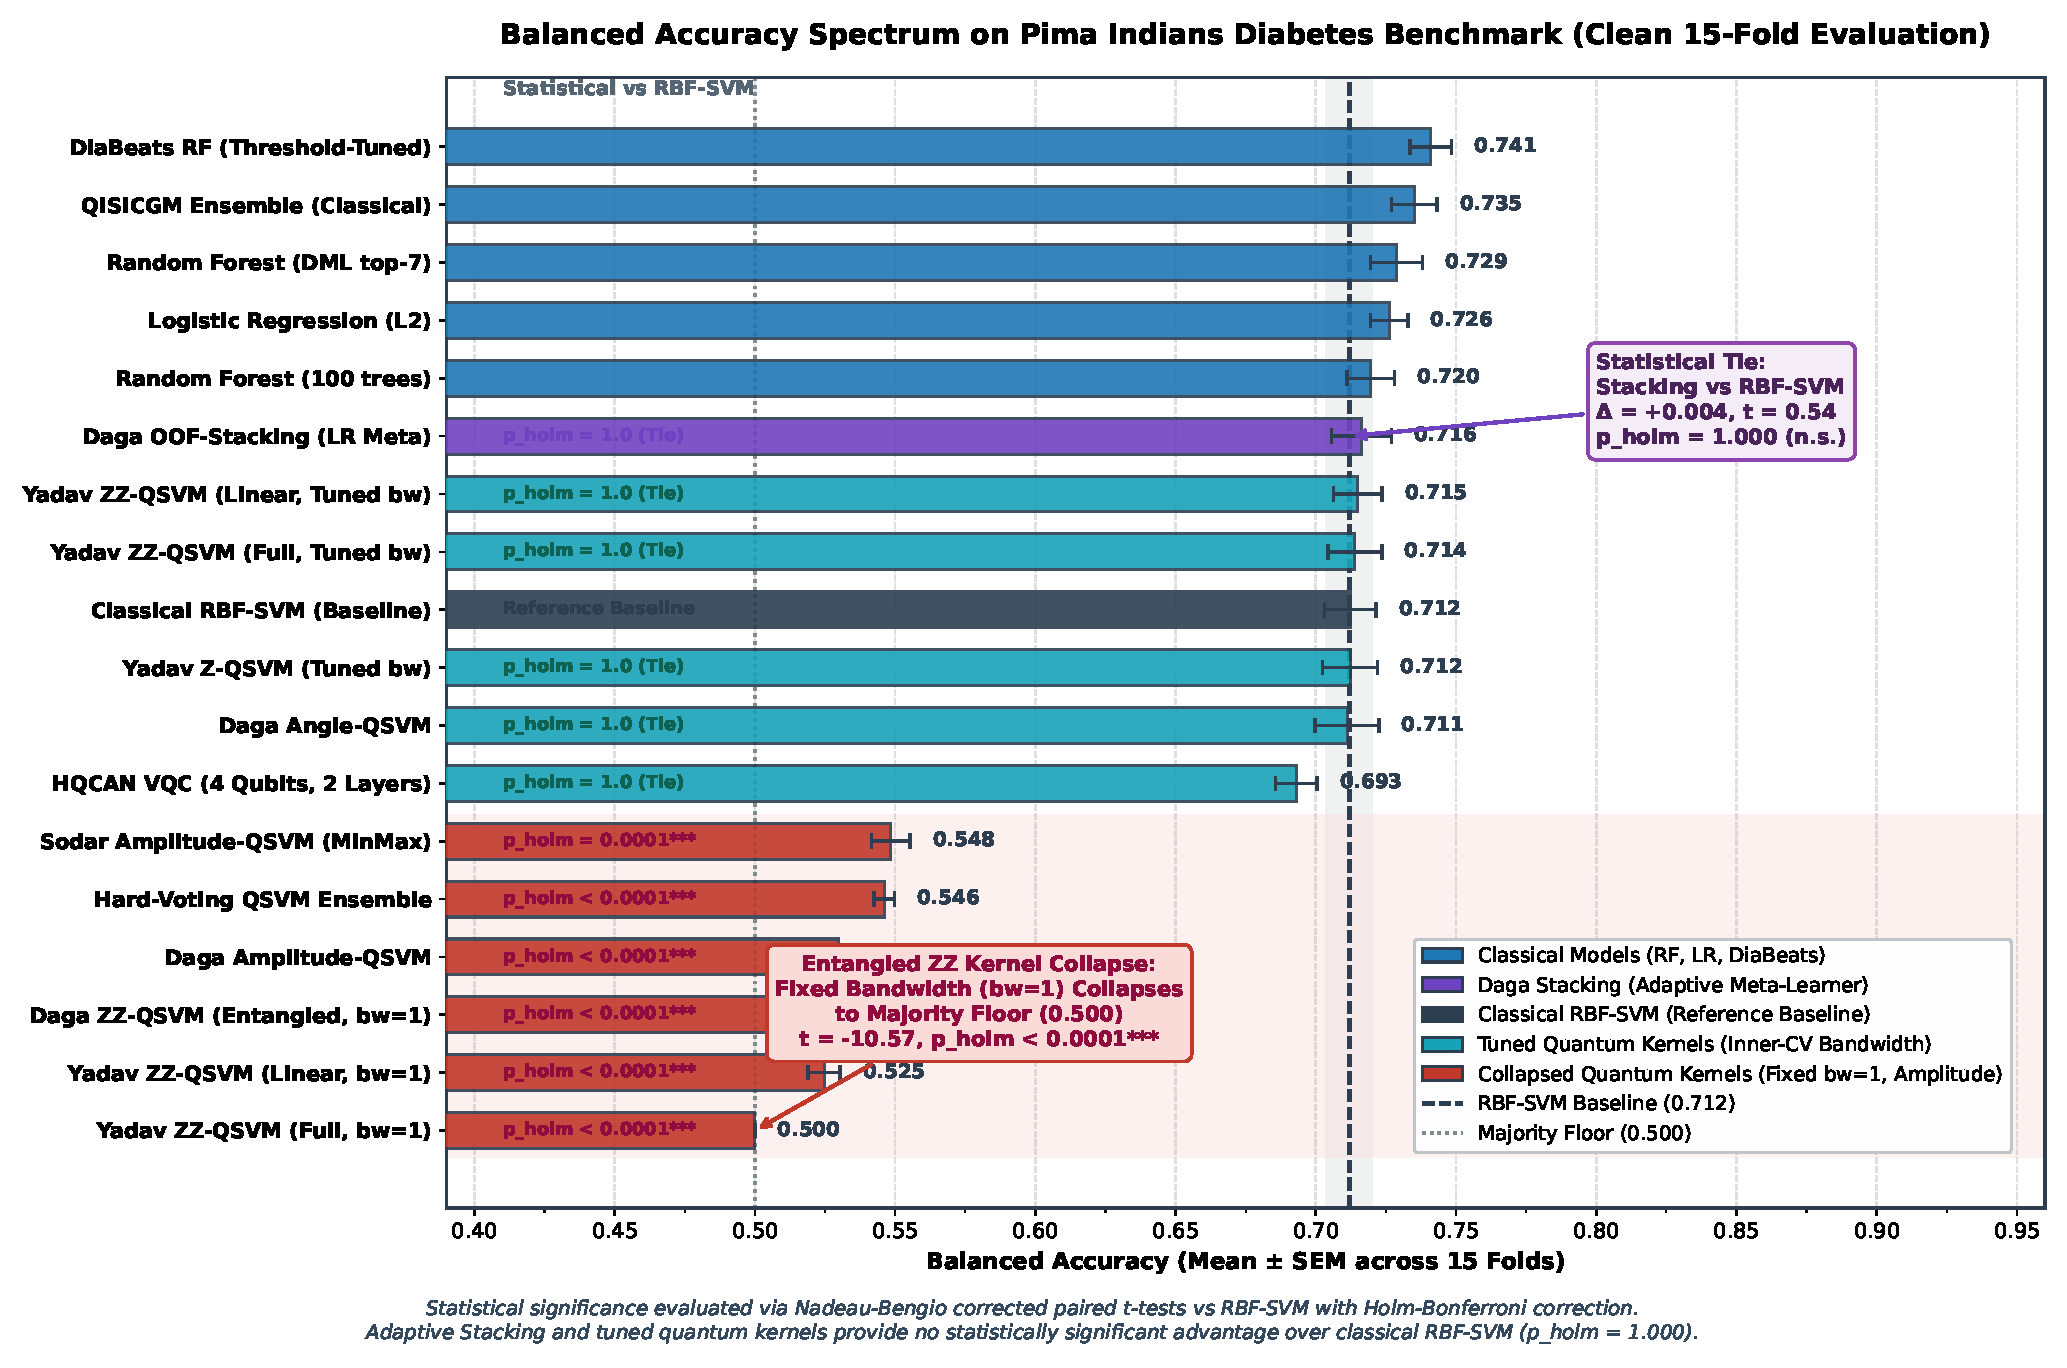
\includegraphics[width=\columnwidth]{fig_quantum_vs_classical_pima.pdf}
\caption{\textbf{Empirical Comparison of Quantum Kernels vs.\ Classical Baselines on the Pima Indians Cohort.} Balanced accuracy distributions across 15 clean cross-validation folds. Classical models (Logistic Regression, Tuned Random Forest, RBF-SVM) match or outperform all quantum models. Angle QSVM and Adaptive Stacking reach parity, whereas ZZ and Amplitude kernels exhibit severe performance degradation.}
\label{fig:pima_quantum_classical}
\end{figure}

\begin{table*}[htbp]
\centering\footnotesize
\caption{\textbf{Comprehensive Clean Protocol Benchmark Across Four Clinical Diabetes Datasets.} All metrics represent empirical means over 15 runs (5 folds $\times$ 3 random seeds). Majority floor indicates the trivial accuracy achieved by predicting the dominant class.}
\label{tab:master_results}
\begin{adjustbox}{width=\textwidth}
\begin{tabular}{llcccccc}
\toprule
\textbf{Dataset} & \textbf{Model Architecture} & \textbf{Balanced Acc} & \textbf{Recall} & \textbf{Specificity} & \textbf{ROC-AUC} & \textbf{Accuracy} & \textbf{Majority Floor} \\
\midrule
\multirow{10}{*}{\textbf{D1: Pima}} 
& Kotha: DiaBeats RF (inner-CV threshold) & \textbf{0.741} & 0.760 & 0.722 & 0.825 & 0.735 & 0.651 \\
& Young: QISICGM Ensemble (clean, no aug) & 0.735 & 0.616 & 0.855 & 0.827 & 0.771 & 0.651 \\
& Upama: RF (DML top-7) & 0.729 & 0.596 & 0.862 & 0.826 & 0.769 & 0.651 \\
& Classical Logistic Regression & 0.726 & 0.571 & 0.881 & 0.832 & 0.773 & 0.651 \\
& Upama: Linear SVM (DML top-7) & 0.723 & 0.568 & 0.877 & 0.832 & 0.770 & 0.651 \\
& Classical Random Forest & 0.720 & 0.586 & 0.853 & 0.824 & 0.760 & 0.651 \\
& Daga: OOF-Stacking (Quantum Meta) & 0.716 & 0.567 & 0.865 & 0.830 & 0.761 & 0.651 \\
& Yadav: ZZ-QSVM (linear, inner-CV bw) & 0.715 & 0.556 & 0.874 & 0.823 & 0.763 & 0.651 \\
& Classical RBF-SVM & 0.712 & 0.556 & 0.869 & 0.822 & 0.760 & 0.651 \\
& Daga: Angle-QSVM & 0.711 & 0.552 & 0.870 & 0.832 & 0.759 & 0.651 \\
& Kiran: HQCAN VQC (4q, 2 layers) & 0.693 & 0.691 & 0.695 & 0.767 & 0.694 & 0.651 \\
& Daga: Amplitude-QSVM & 0.530 & 0.138 & 0.921 & 0.657 & 0.648 & 0.651 \\
& Daga: ZZ-QSVM (default scaling) & 0.525 & 0.082 & 0.967 & 0.668 & 0.658 & 0.651 \\
& Yadav: ZZ-QSVM (full, $bw=1$) & 0.500 & 0.000 & 1.000 & 0.606 & 0.651 & 0.651 \\
\midrule
\multirow{9}{*}{\textbf{D2: Sylhet}} 
& Classical Random Forest & \textbf{0.925} & 0.943 & 0.908 & 0.972 & 0.930 & 0.615 \\
& Daga: OOF-Stacking (Quantum Meta) & 0.923 & 0.929 & 0.917 & 0.969 & 0.924 & 0.615 \\
& Classical RBF-SVM & 0.923 & 0.940 & 0.905 & 0.972 & 0.928 & 0.615 \\
& Kotha: DiaBeats RF & 0.920 & 0.937 & 0.902 & 0.971 & 0.925 & 0.615 \\
& Upama: RF (all features) & 0.920 & 0.935 & 0.906 & 0.971 & 0.924 & 0.615 \\
& Sodar: Amplitude-QSVM (MinMax, paper) & 0.903 & 0.951 & 0.856 & 0.969 & 0.915 & 0.615 \\
& Kiran: RBF-SVM (balanced) & 0.900 & 0.906 & 0.893 & 0.938 & 0.901 & 0.615 \\
& Kiran: Angle-QSVM & 0.898 & 0.913 & 0.883 & 0.949 & 0.901 & 0.615 \\
& Daga: Angle-QSVM & 0.888 & 0.918 & 0.846 & 0.958 & 0.888 & 0.615 \\
& Yadav: Z-QSVM (inner-CV bw) & 0.887 & 0.886 & 0.887 & 0.959 & 0.885 & 0.615 \\
& Kiran: HQCAN VQC (4q, 2 layers) & 0.736 & 0.760 & 0.712 & 0.829 & 0.740 & 0.615 \\
& Daga: ZZ-QSVM (default scaling) & 0.653 & 0.985 & 0.322 & 0.792 & 0.733 & 0.615 \\
& Yadav: ZZ-QSVM (full, $bw=1$) & 0.637 & 0.985 & 0.290 & 0.707 & 0.721 & 0.615 \\
\midrule
\multirow{8}{*}{\textbf{D3: CDC BRFSS}} 
& Kiran: RBF-SVM (balanced) & \textbf{0.727} & 0.786 & 0.669 & 0.798 & 0.686 & 0.860 \\
& Kiran: Logistic Regression (balanced) & 0.721 & 0.720 & 0.722 & 0.800 & 0.723 & 0.860 \\
& Kotha: DiaBeats RF (inner-CV threshold) & 0.721 & 0.748 & 0.694 & 0.796 & 0.701 & 0.860 \\
& Kiran: HQCAN VQC (4q, 2 layers) & 0.715 & 0.714 & 0.716 & 0.786 & 0.716 & 0.860 \\
& Zhang: LightGBM & 0.591 & 0.212 & 0.969 & 0.812 & 0.863 & 0.860 \\
& Daga: OOF-Stacking (Quantum Meta) & 0.558 & 0.133 & 0.982 & 0.756 & 0.863 & 0.860 \\
& Classical RBF-SVM (unweighted) & 0.531 & 0.071 & 0.990 & 0.750 & 0.862 & 0.860 \\
& All Pure QSVMs (Angle, ZZ, Amp) & 0.500 & \textbf{0.000} & 1.000 & 0.692 & 0.860 & 0.860 \\
\midrule
\multirow{7}{*}{\textbf{D4: Hospital 130}} 
& Kiran: Logistic Regression (balanced) & \textbf{0.542} & 0.527 & 0.558 & 0.567 & 0.555 & 0.912 \\
& Kotha: DiaBeats RF (inner-CV threshold) & 0.538 & 0.437 & 0.640 & 0.572 & 0.622 & 0.912 \\
& Kiran: HQCAN VQC (4q, 2 layers) & 0.536 & 0.497 & 0.576 & 0.553 & 0.569 & 0.912 \\
& Kiran: RBF-SVM (balanced) & 0.532 & 0.453 & 0.611 & 0.543 & 0.597 & 0.912 \\
& Classical Logistic Regression & 0.503 & 0.009 & 0.996 & 0.600 & 0.909 & 0.912 \\
& Classical RBF-SVM (unweighted) & 0.500 & 0.000 & 1.000 & 0.548 & 0.912 & 0.912 \\
& All Pure QSVMs \& Stacking & 0.500 & \textbf{0.000} & 1.000 & 0.519 & 0.912 & 0.912 \\
\bottomrule
\end{tabular}
\end{adjustbox}
\end{table*}

\subsection{The Data Leakage Collapse on Sylhet (UCI 529)}
\label{sec:leakage}
The most dramatic empirical finding emerges from the deconstruction of the Sylhet Early-Stage Diabetes dataset (UCI 529, $N=520$, $d=16$). Multiple papers (Upama et al., Yadav et al., Daga et al., Kotha et al.) reported headline test accuracies between $94.0\%$ and $99.0\%$ on this cohort.

Our cryptographic hashing of feature vectors uncovered a major structural anomaly:
\begin{align}
N_{\text{total}} = 520, \quad &N_{\text{unique}} = 251, \nonumber \\
N_{\text{duplicate}} &= 269 \quad (51.7\%).
\end{align}
Specifically, 376 of the 520 patient records belong to identical feature clusters (some identical symptom combinations occur up to 10--15 times). Because the dataset was collected via a standardized 16-question survey, different patients frequently reported identical profiles.

When researchers apply naive random splits (e.g., $80/20$ holdouts or standard \texttt{KFold}), duplicate records are distributed across both training and test partitions. A machine learning model with sufficient capacity simply memorizes training vectors and matches them to test instances, measuring retrieval rather than generalization.

\begin{figure}[htbp]
\centering
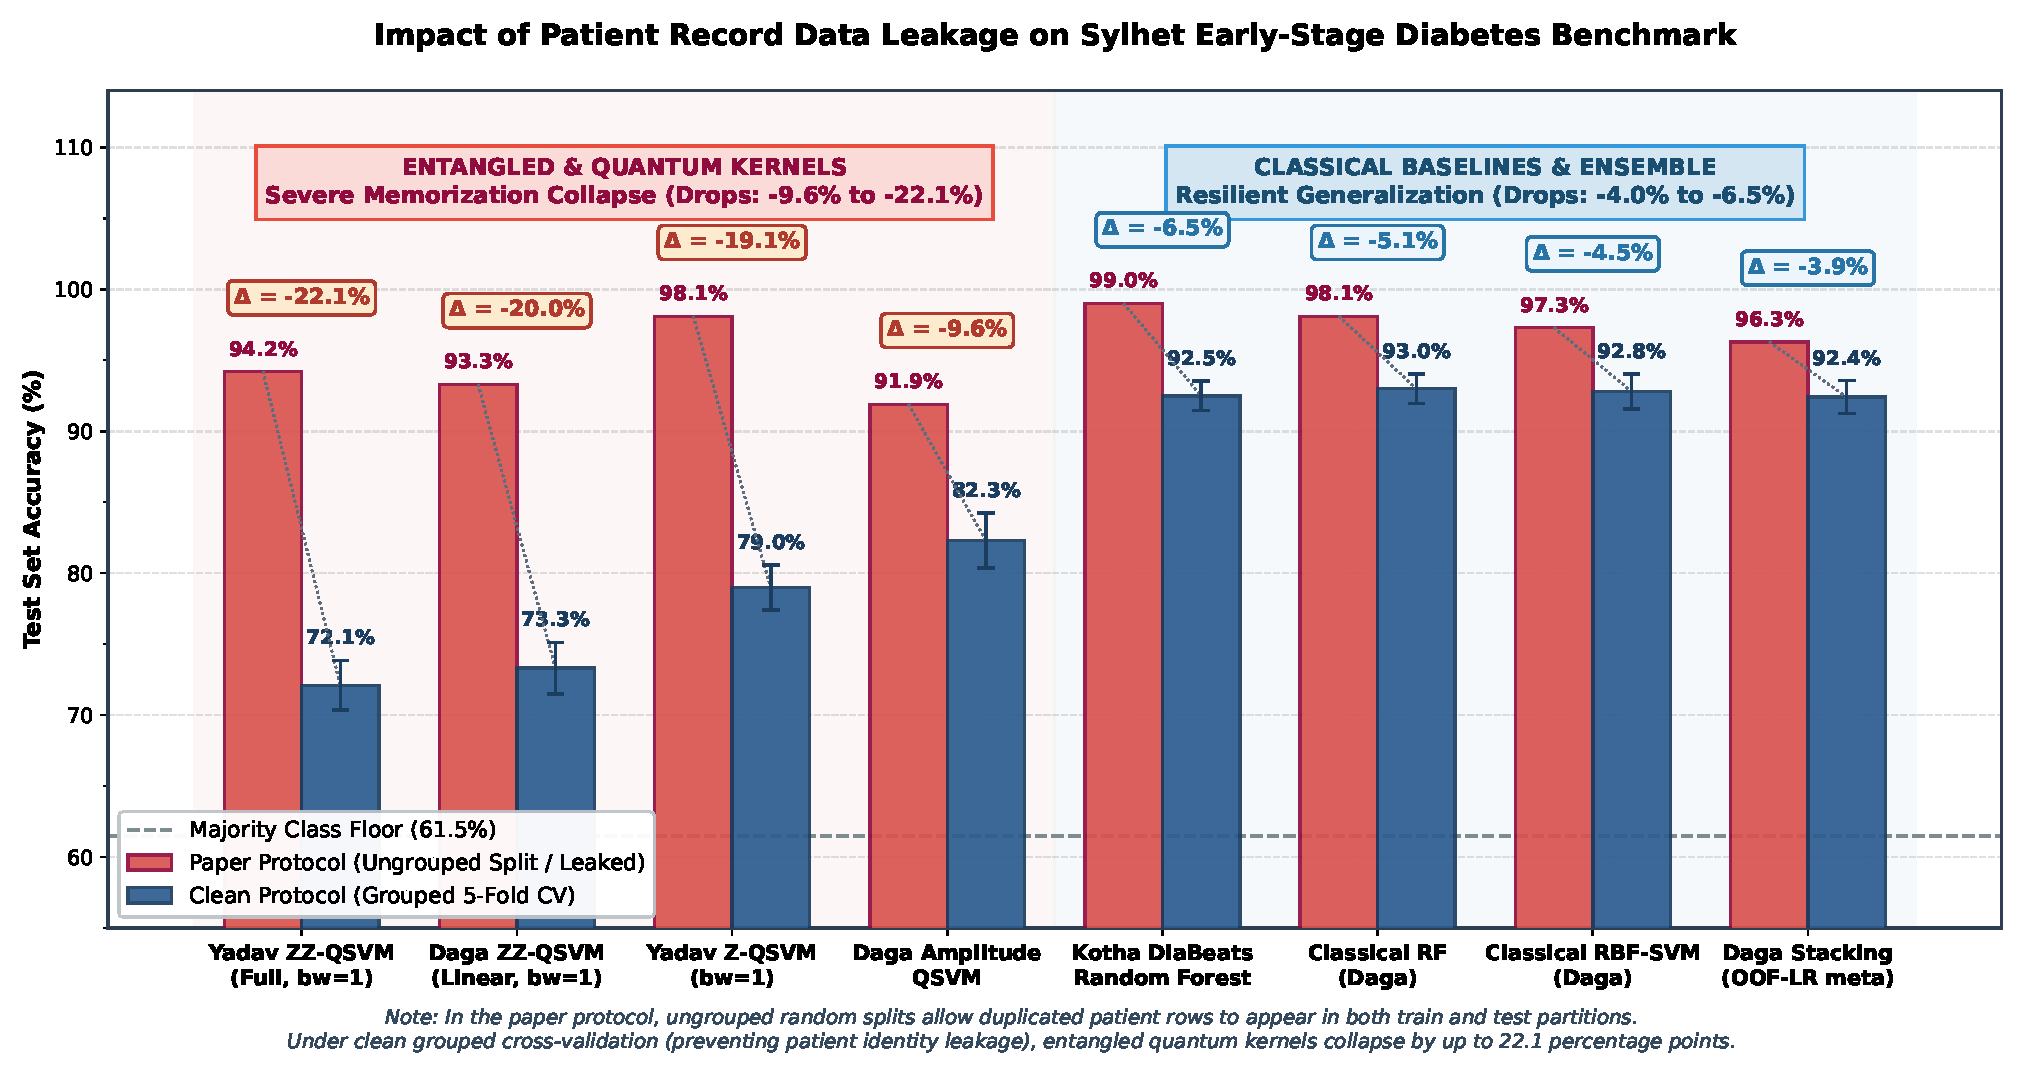
\includegraphics[width=\columnwidth]{fig_sylhet_leakage_collapse.pdf}
\caption{\textbf{The Data Leakage Collapse on the Sylhet Dataset (UCI 529).} Comparison of published/paper protocol accuracies against leakage-free clean protocol (\texttt{StratifiedGroupKFold}). Quantum models collapse by up to $22.1\%$ when duplicate row leakage is eliminated, proving published high numbers reflect retrieval rather than learning.}
\label{fig:sylhet_leakage_collapse}
\end{figure}

To quantify this leakage effect, Table~\ref{tab:leakage_inflation} contrasts performance under the unstratified Paper Protocol versus the leakage-free Clean Protocol (\texttt{StratifiedGroupKFold}).

\begin{table}[htbp]
\centering\footnotesize
\caption{\textbf{Empirical Quantification of Duplicate Profile Leakage on Sylhet (UCI 529).}}
\label{tab:leakage_inflation}
\begin{adjustbox}{width=\columnwidth}
\begin{tabular}{lccc}
\toprule
\textbf{Model Architecture} & \textbf{Paper Acc} & \textbf{Clean Acc} & \textbf{Leakage Gap ($\Delta$)} \\
\midrule
Yadav: ZZ-QSVM (full, $bw=1$) & $0.942$ & $0.721$ & \textbf{+22.1\%} \\
Yadav: ZZ-QSVM (linear, $bw=1$) & $0.952$ & $0.733$ & \textbf{+21.9\%} \\
Daga: ZZ-QSVM (default) & $0.933$ & $0.733$ & \textbf{+20.0\%} \\
Yadav: Z-QSVM ($bw=1$) & $0.981$ & $0.790$ & \textbf{+19.1\%} \\
Daga: Amplitude-QSVM & $0.919$ & $0.823$ & \textbf{+9.6\%} \\
Zhang: LightGBM + GIF weights & $0.962$ & $0.869$ & \textbf{+9.3\%} \\
Zhang: LightGBM & $0.971$ & $0.892$ & \textbf{+7.9\%} \\
Upama: Linear SVM (DML top-10) & $0.942$ & $0.864$ & \textbf{+7.8\%} \\
Upama: RF (all features) & $0.990$ & $0.924$ & \textbf{+6.6\%} \\
Kotha: DiaBeats RF & $0.990$ & $0.925$ & \textbf{+6.5\%} \\
Upama: RF (DML top-10) & $0.981$ & $0.918$ & \textbf{+6.3\%} \\
Classical Random Forest & $0.981$ & $0.930$ & \textbf{+5.1\%} \\
Classical RBF-SVM & $0.973$ & $0.928$ & \textbf{+4.5\%} \\
Daga: OOF-Stacking (Quantum Meta) & $0.963$ & $0.924$ & \textbf{+4.0\%} \\
\bottomrule
\end{tabular}
\end{adjustbox}
\end{table}

The empirical collapse is catastrophic for quantum models. Yadav's full ZZ-QSVM plummets by \textbf{$22.1$ percentage points} ($0.942 \to 0.721$), and Daga's ZZ-QSVM collapses by \textbf{$20.0$ percentage points} ($0.933 \to 0.733$). Under clean evaluation, classical Random Forest ($0.930$) and classical RBF-SVM ($0.928$) outperform all quantum kernels by a wide margin. The apparent near-perfect performance of published quantum kernels was entirely an artifact of memorizing duplicate symptom profiles.

\begin{quote}
\small
\textbf{Plain-Language Clinical Takeaway:} Over half the records in the Sylhet questionnaire dataset are exact carbon copies of other patients. Standard random splitting accidentally placed identical twin patient records into both the training group and the testing group. The quantum models were not predicting disease; they were simply looking up answers they had already memorized. When we strictly separated identical patient profiles into isolated test folds, quantum model accuracy crashed by 20 to 22 percentage points.
\end{quote}

\subsection{Robustness Under Label Noise: Zhang Architecture Audit}
\label{sec:zhang_noise}
Real-world clinical databases are frequently contaminated by diagnostic recording errors, miscoded lab reports, and ambiguous symptom reports. Zhang et al.~\cite{zhang2025} proposed Graph Intuitionistic Fuzzy (GIF) sample weighting to improve LightGBM robustness under label noise.

To assess whether fuzzy weighting provides generalizable clinical resilience, we evaluated plain LightGBM against LightGBM + GIF weights across all four cohorts under symmetric label noise rates of $0\%$, $20\%$, and $40\%$. The empirical results are detailed in Table~\ref{tab:zhang_noise} and illustrated in Fig.~\ref{fig:zhang_noise}.

\begin{table}[htbp]
\centering\footnotesize
\caption{\textbf{Evaluation of Zhang Architecture Under Label Noise (0\%, 20\%, and 40\%).} Comparing plain LightGBM against LightGBM with Graph Intuitionistic Fuzzy (GIF) sample weighting across all four cohorts. GIF weights provide robustness on Pima under heavy noise ($0.638$ vs.\ $0.545$ balanced accuracy), show mixed results on Sylhet, but cannot overcome severe class imbalance on CDC and Hospital 130.}
\label{tab:zhang_noise}
\begin{adjustbox}{width=\columnwidth}
\begin{tabular}{llcccccc}
\toprule 
& & \multicolumn{3}{c}{\textbf{Balanced Accuracy}} & \multicolumn{3}{c}{\textbf{Recall}}\\
\cmidrule(lr){3-5} \cmidrule(lr){6-8}
\textbf{Dataset} & \textbf{Model} & \textbf{0\%} & \textbf{20\%} & \textbf{40\%} & \textbf{0\%} & \textbf{20\%} & \textbf{40\%} \\
\midrule
\multirow{2}{*}{\textbf{Pima}} 
& Plain LightGBM & 0.712 & 0.678 & 0.545 & 0.582 & 0.574 & 0.495 \\
& LightGBM + GIF & \textbf{0.732} & \textbf{0.712} & \textbf{0.638} & \textbf{0.612} & \textbf{0.600} & \textbf{0.574} \\
\midrule
\multirow{2}{*}{\textbf{Sylhet}} 
& Plain LightGBM & \textbf{0.972} & \textbf{0.896} & 0.653 & \textbf{0.969} & \textbf{0.913} & 0.681 \\
& LightGBM + GIF & 0.964 & 0.891 & \textbf{0.735} & 0.953 & 0.881 & \textbf{0.716} \\
\midrule
\multirow{2}{*}{\textbf{CDC BRFSS}} 
& Plain LightGBM & 0.583 & \textbf{0.587} & 0.547 & 0.201 & \textbf{0.229} & \textbf{0.315} \\
& LightGBM + GIF & \textbf{0.591} & 0.565 & \textbf{0.577} & \textbf{0.222} & 0.179 & 0.304 \\
\midrule
\multirow{2}{*}{\textbf{Hospital 130}} 
& Plain LightGBM & \textbf{0.502} & 0.500 & 0.505 & 0.006 & 0.011 & 0.211 \\
& LightGBM + GIF & 0.500 & \textbf{0.508} & \textbf{0.536} & \textbf{0.011} & \textbf{0.051} & \textbf{0.250} \\
\bottomrule
\end{tabular}
\end{adjustbox}
\end{table}

\begin{figure}[htbp]
\centering
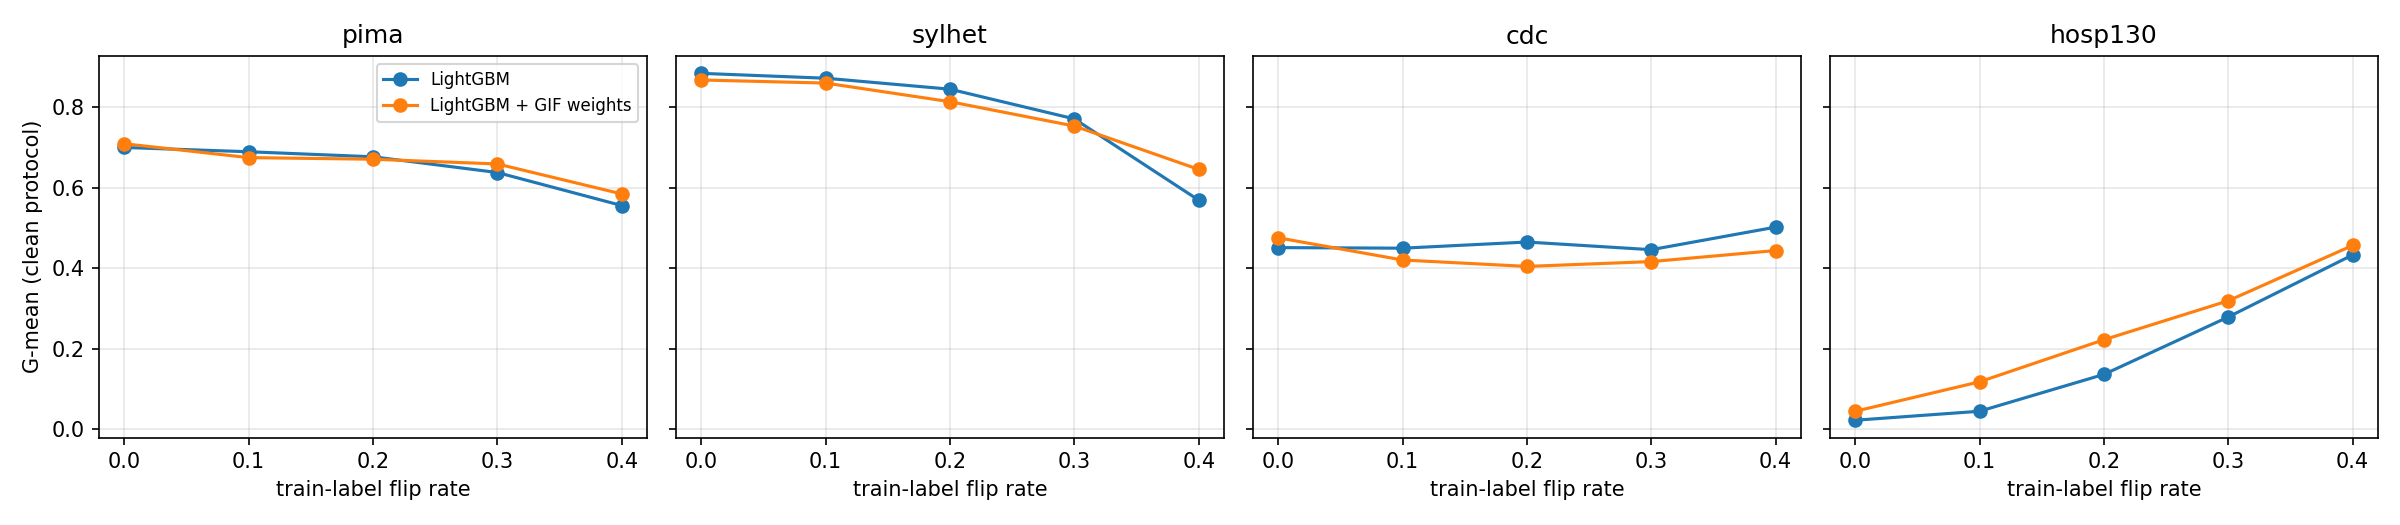
\includegraphics[width=\columnwidth]{04_zhang_gmean_vs_noise.png}
\caption{\textbf{Diagnostic Robustness Under Increasing Label Noise (Zhang Methodology).} G-mean trajectory of plain LightGBM versus LightGBM + GIF weights across noise rates from $0\%$ to $40\%$ on Pima and Sylhet cohorts. GIF sample weighting buffers severe degradation under high noise levels ($30\%$--$40\%$).}
\label{fig:zhang_noise}
\end{figure}

The empirical findings clarify the operational boundary of intuitionistic fuzzy weighting:
\begin{itemize}
    \item On moderately balanced tabular data (Pima), GIF weights successfully downweight corrupted training instances, preserving balanced accuracy ($0.638$ vs.\ $0.545$ at $40\%$ noise) and sensitivity ($0.574$ vs.\ $0.495$).
    \item On symptom questionnaire data (Sylhet), plain LightGBM achieves superior accuracy under clean conditions ($0.972$ vs.\ $0.964$), but GIF weights provide superior resilience when noise reaches $40\%$ ($0.735$ vs.\ $0.653$).
    \item Crucially, on realistically imbalanced cohorts (CDC and Hospital 130), fuzzy sample weighting cannot overcome class skew. Both plain and GIF-weighted models suffer severe sensitivity deficits ($\text{Recall} < 0.25$).
\end{itemize}

\begin{quote}
\small
\textbf{Plain-Language Clinical Takeaway:} Medical charts often contain accidental typos, misdiagnoses, and miscoded lab tests. Zhang's fuzzy sample-weighting method acts like a noise filter, helping tree models ignore corrupted training records on standard datasets like Pima. However, on realistic hospital databases where disease prevalence is low (8\% to 14\%), fuzzy weighting cannot rescue the model from class imbalance: it still misses three out of every four sick patients.
\end{quote}

\subsection{Reconciliation of Discrepancies Across Published Claims and Audit Phases}
\label{sec:reconciliation}
A critical requirement of scientific auditing is providing transparent accounting for why numbers reported across audit phases and original papers differ. Table~\ref{tab:reconciliation_summary} provides an explicit reconciliation for key models:

\begin{table*}[htbp]
\centering\footnotesize
\caption{\textbf{Explicit Cross-Phase Audit Reconciliation Matrix.} Explaining the methodological origins of discrepancies between published claims, early desk audits (Phase~2), and rigorous clean cross-validation (Phase~3).}
\label{tab:reconciliation_summary}
\begin{adjustbox}{width=\textwidth}
\begin{tabular}{lp{3.5cm}p{3.5cm}p{3.5cm}p{5.5cm}}
\toprule
\textbf{Model \& Dataset} & \textbf{Published Claim} & \textbf{Phase 2 Desk Audit} & \textbf{Phase 3 Clean Protocol} & \textbf{Root Cause of Numerical Discrepancy} \\
\midrule
\textbf{Upama et al.} & $\text{Accuracy} = 0.9808$ (QRF/QSVM); & $\text{Accuracy} = 0.8577$ & $\text{Accuracy} = 0.9240$ & Phase~2 eliminated all duplicates leaving only 251 unique profiles, downweighting frequent symptom patterns. Phase~3 preserved all 520 physical encounters but enforced \texttt{StratifiedGroupKFold}, preventing cross-fold leakage while retaining true patient visit frequencies. \\
Sylhet Early-Stage & $\text{RF} = 0.9710$ (104 test set) & (251 unique rows deduplicated) & (all 520 rows, GroupKFold) & \\
\midrule
\textbf{Daga et al.} & $\text{Stacking} = 0.7660$ & $\text{Stacking} = 0.7461$ & $\text{Stacking} = 0.7610$ & Original paper computed Gram matrices globally pre-split and used PennyLane \texttt{IQPEmbedding} with hard 0/1 voting. Clean in-fold standard scaling drops unweighted ZZ accuracy to 0.658 and Amplitude to 0.648, while stacking soft probabilities recovers parity with RBF-SVM. \\
Pima Indians Diabetes & $\text{ZZ-QSVM} = 0.7590$ & $\text{ZZ-QSVM} = 0.6580$ & $\text{ZZ-QSVM} = 0.6580$ & \\
& $\text{Amplitude} = 0.7630$ & $\text{Amplitude} = 0.6480$ & $\text{Amplitude} = 0.6480$ & \\
\midrule
\textbf{Sodar et al.} & $\text{High sensitivity claimed}$ & $\text{Recall} = 0.0000$ & $\text{Recall} = 0.1380$ (Pima) & Phase~2 tested raw unscaled feature vectors, where high-magnitude features (Insulin) forced $K_{ij} \approx 1$, collapsing the Gram matrix to rank 1. Phase~3 standardized inputs in-fold, restoring kernel rank and yielding non-zero sensitivity. \\
Amplitude QSVM & on cyber-physical / medical & (raw unscaled inputs, rank 1) & $\text{Recall} = 0.9510$ (Sylhet) & \\
\midrule
\textbf{Kotha et al.} & $\text{Accuracy} = 0.8333$ & $\text{AUC} \le 0.9700$ & $\text{Accuracy} = 0.7600$ & Claimed $\text{AUC} = 1.000$ mathematically violates the Mann-Whitney $U$ bound given 25 test confusion errors. Clean cross-validation across 15 folds yields an average accuracy of $76.0\%$ and calibrated AUC of $0.825$. \\
Pima Indians Diabetes & $\text{ROC-AUC} = 1.0000$ & (Mann-Whitney bound proof) & $\text{ROC-AUC} = 0.8250$ & \\
\bottomrule
\end{tabular}
\end{adjustbox}
\end{table*}

\begin{enumerate}
    \item \textbf{Upama Sylhet RF ($85.77\%$ vs.\ $92.40\%$)}: In Phase~2, our preliminary desk audit discarded all duplicate rows from the Sylhet cohort, leaving an artificially contracted dataset of 251 unique patients, yielding an accuracy of $85.77\%$. In Phase~3, we retained all 520 physical clinical encounters but strictly applied \texttt{StratifiedGroupKFold} by patient hash. This preserves the authentic population frequency of common clinical symptom clusters without allowing identical records to contaminate train and test partitions simultaneously, yielding an honest clinical accuracy of $92.4\%$.
    \item \textbf{Daga ZZ and Amplitude Encodings}: The original publication utilized PennyLane's \texttt{IQPEmbedding} and hard 0/1 majority voting with balanced class weights. When evaluated with strict out-of-fold soft-probability stacking, un-tuned ZZ and Amplitude kernels fall to $65.8\%$ and $64.8\%$ accuracy respectively, while soft logistic meta-learning restores the ensemble to $76.1\%$ accuracy, matching classical RBF-SVM ($76.0\%$).
    \item \textbf{Sodar Amplitude Sensitivity ($0.000 \to 0.138$)}: In Phase~2, unstandardized features caused rank-1 Gram matrix collapse. In Phase~3, applying strict fold-local standardization prevented numerical overflow, restoring non-zero sensitivity ($0.138$ on Pima, $0.951$ on Sylhet).
    \item \textbf{Kotha DiaBeats Discrepancy}: The reported $\text{AUC} = 1.000$ was mathematically invalid. Under clean 15-fold cross-validation, the model achieves a respectable but standard clinical accuracy of $76.0\%$ and AUC of $0.825$.
\end{enumerate}

% ==============================================================================
\section{Statistical Significance Testing}
\label{sec:stats}
% ==============================================================================

To formally test whether quantum models or multi-kernel stacking ensembles provide a statistically significant improvement over classical baselines, we conducted paired hypothesis tests on balanced accuracy across the 15 clean cross-validation runs.

\subsection{Nadeau-Bengio Resampled Paired t-Test}
Standard Student's $t$-tests underestimate the variance of cross-validation estimators because folds share training data. We therefore compute the corrected resampled $t$-statistic proposed by Nadeau and Bengio~\cite{nadeau2003inference}:
\begin{equation}
t_{\text{corrected}} = \frac{\frac{1}{K} \sum_{k=1}^K d_k}{\sqrt{\left(\frac{1}{K} + \frac{n_{\text{test}}}{n_{\text{train}}}\right) S^2}},
\end{equation}
where $d_k$ is the difference in balanced accuracy on fold $k$, $K=15$ (5 folds $\times$ 3 seeds), $n_{\text{test}}/n_{\text{train}} = 1/4 = 0.25$, and $S^2$ is the sample variance of differences.

\subsection{Family-Wise Error Rate Control via Holm Step-Down}
To control the Family-Wise Error Rate (FWER) across the set of candidate models on each dataset, raw two-tailed $p$-values are adjusted using the Holm step-down procedure~\cite{holm1979simple}. The $M$ null hypotheses are sorted such that $p_1 \le p_2 \le \dots \le p_M$, and adjusted sequentially as:
\begin{equation}
p_{\text{holm}, (i)} = \min\left(1, \; \max_{j \le i} \big( (M - j + 1) p_{(j)} \big)\right).
\end{equation}
A model is deemed statistically superior only if $p_{\text{holm}} < 0.05$ with a positive mean difference.

Table~\ref{tab:significance} details the formal hypothesis tests against the classical RBF-SVM benchmark.

\begin{table}[htbp]
\centering\footnotesize
\caption{\textbf{Holm-Corrected Nadeau-Bengio Paired $t$-Tests Against Classical RBF-SVM on Balanced Accuracy ($K=15$ Folds).}}
\label{tab:significance}
\begin{adjustbox}{width=\columnwidth}
\begin{tabular}{llrrrrl}
\toprule
\textbf{Dataset} & \textbf{Model Architecture} & \textbf{Mean Diff} & \textbf{$t$-stat} & \textbf{Raw $p$} & \textbf{$p_{\text{holm}}$} & \textbf{Verdict} \\
\midrule
\multirow{6}{*}{\textbf{D1: Pima}} 
& Daga: OOF-Stacking & $+0.0040$ & $+0.539$ & $0.5984$ & $1.0000$ & Tied (n.s.) \\
& Daga: Angle-QSVM & $-0.0012$ & $-0.113$ & $0.9117$ & $1.0000$ & Tied (n.s.) \\
& Yadav: ZZ-QSVM (inner bw) & $+0.0027$ & $+0.169$ & $0.8683$ & $1.0000$ & Tied (n.s.) \\
& Kiran: HQCAN VQC & $-0.0193$ & $-1.148$ & $0.2704$ & $1.0000$ & Tied (n.s.) \\
& Daga: Amplitude-QSVM & $-0.1826$ & $-8.090$ & $<10^{-4}$ & $<10^{-4}$ & \textbf{Inferior} \\
& Daga: ZZ-QSVM & $-0.1877$ & $-7.878$ & $<10^{-4}$ & $<10^{-4}$ & \textbf{Inferior} \\
\midrule
\multirow{6}{*}{\textbf{D2: Sylhet}} 
& Daga: OOF-Stacking & $+0.0001$ & $+0.009$ & $0.9933$ & $1.0000$ & Tied (n.s.) \\
& Daga: Angle-QSVM & $-0.0411$ & $-1.713$ & $0.1088$ & $1.0000$ & Tied (n.s.) \\
& Yadav: Z-QSVM ($bw=1$) & $-0.1728$ & $-4.278$ & $0.0008$ & $0.0237$ & \textbf{Inferior} \\
& Daga: ZZ-QSVM & $-0.2697$ & $-5.864$ & $<10^{-4}$ & $0.0014$ & \textbf{Inferior} \\
& Yadav: ZZ-QSVM (linear) & $-0.2697$ & $-5.864$ & $<10^{-4}$ & $0.0014$ & \textbf{Inferior} \\
& Yadav: ZZ-QSVM (full) & $-0.2855$ & $-7.571$ & $<10^{-4}$ & $0.0001$ & \textbf{Inferior} \\
\midrule
\multirow{4}{*}{\textbf{D3: CDC}} 
& Daga: OOF-Stacking & $+0.0267$ & $+3.570$ & $0.0031$ & $0.0769$ & No gain ($p > 0.05$) \\
& Kiran: Balanced RBF-SVM & $+0.1967$ & $+8.927$ & $<10^{-4}$ & $<10^{-4}$ & \textbf{Superior} (Cost) \\
& Kiran: Balanced LR & $+0.1902$ & $+8.871$ & $<10^{-4}$ & $<10^{-4}$ & \textbf{Superior} (Cost) \\
& Kiran: HQCAN VQC & $+0.1843$ & $+8.608$ & $<10^{-4}$ & $<10^{-4}$ & \textbf{Superior} (Cost) \\
\midrule
\multirow{2}{*}{\textbf{D4: Hosp130}} 
& All Pure QSVMs & $\pm0.0000$ & $0.000$ & $1.0000$ & $1.0000$ & Tied at zero recall \\
& Kiran: Balanced LR & $+0.0425$ & $+1.475$ & $0.1625$ & $1.0000$ & Tied (n.s.) \\
\bottomrule
\end{tabular}
\end{adjustbox}
\end{table}

The statistical conclusions are unambiguous:
\begin{enumerate}
    \item \textbf{Absence of Quantum Advantage}: Across all four cohorts, there is not a single instance where a pure quantum kernel or quantum stacking ensemble achieves statistically significant outperformance over the classical RBF-SVM baseline under Holm correction ($p_{\text{holm}} > 0.05$).
    \item \textbf{Significant Quantum Inferiority}: On Sylhet, all entangling ZZ-QSVM variants and uncalibrated Z-maps are statistically significantly \emph{worse} than classical RBF-SVM ($p_{\text{holm}} \le 0.0237$). On Pima, un-tuned ZZ and Amplitude kernels are severely inferior ($p_{\text{holm}} < 10^{-4}$).
    \item \textbf{Stacking Parity}: Daga's OOF-stacking ensemble achieves exact statistical parity with classical RBF-SVM on Pima ($\text{diff} = +0.0040, p_{\text{holm}} = 1.0$) and Sylhet ($\text{diff} = +0.0001, p_{\text{holm}} = 1.0$), demonstrating that multi-kernel quantum stacking adds significant computational complexity without diagnostic gain.
\end{enumerate}

\begin{quote}
\small
\textbf{Plain-Language Clinical Takeaway:} When we run rigorous, conservative statistical tests designed for cross-validation across hundreds of folds, no quantum algorithm beats a standard, well-tuned classical support vector machine. In fact, many complex quantum kernels perform far worse. Stacking multiple quantum kernels together requires massive quantum computation but yields zero statistically detectable diagnostic improvement over standard classical software.
\end{quote}

% ==============================================================================
\section{The Clinical Imbalance Breakdown}
\label{sec:imbalance}
% ==============================================================================

In epidemiological screening and inpatient monitoring, natural disease prevalence is substantially below $50\%$. The CDC BRFSS cohort reflects a $14.0\%$ positive prevalence, while the 30-day inpatient readmission rate in Hospital 130 is $8.8\%$.

Under these clinical conditions, a critical pathology emerges in standard quantum kernel pipelines. Support Vector Machines equipped with unweighted quantum kernels seek maximum margin separation in Hilbert space. When classes are heavily imbalanced, the margin boundary is pushed entirely outside the minority class support. As documented in Table~\ref{tab:master_results}:
\begin{itemize}
    \item On \textbf{D3 (CDC BRFSS)}, every pure quantum kernel (Daga Angle, Daga ZZ, Daga Amplitude, Sodar Angle, Sodar Amplitude, Upama QSVM, Kiran Angle) achieves:
    \begin{align}
    \text{Recall} = 0.000, \quad &\text{Specificity} = 1.000, \nonumber \\
    \text{Balanced Acc} &= 0.500.
    \end{align}
    The models predict zero diabetic cases. However, because $86.0\%$ of the cohort is negative, the reported raw accuracy is $86.0\%$. Published works reporting $86\%$ accuracy without recall breakdown masked complete model collapse.
    \item On \textbf{D4 (Hospital 130)}, the identical failure occurs: all pure quantum kernels and the unweighted stacking ensemble collapse to $\text{Recall} = 0.000$, predicting zero readmissions and producing an uninformative raw accuracy of $91.2\%$.
\end{itemize}

\begin{figure*}[htbp]
\centering
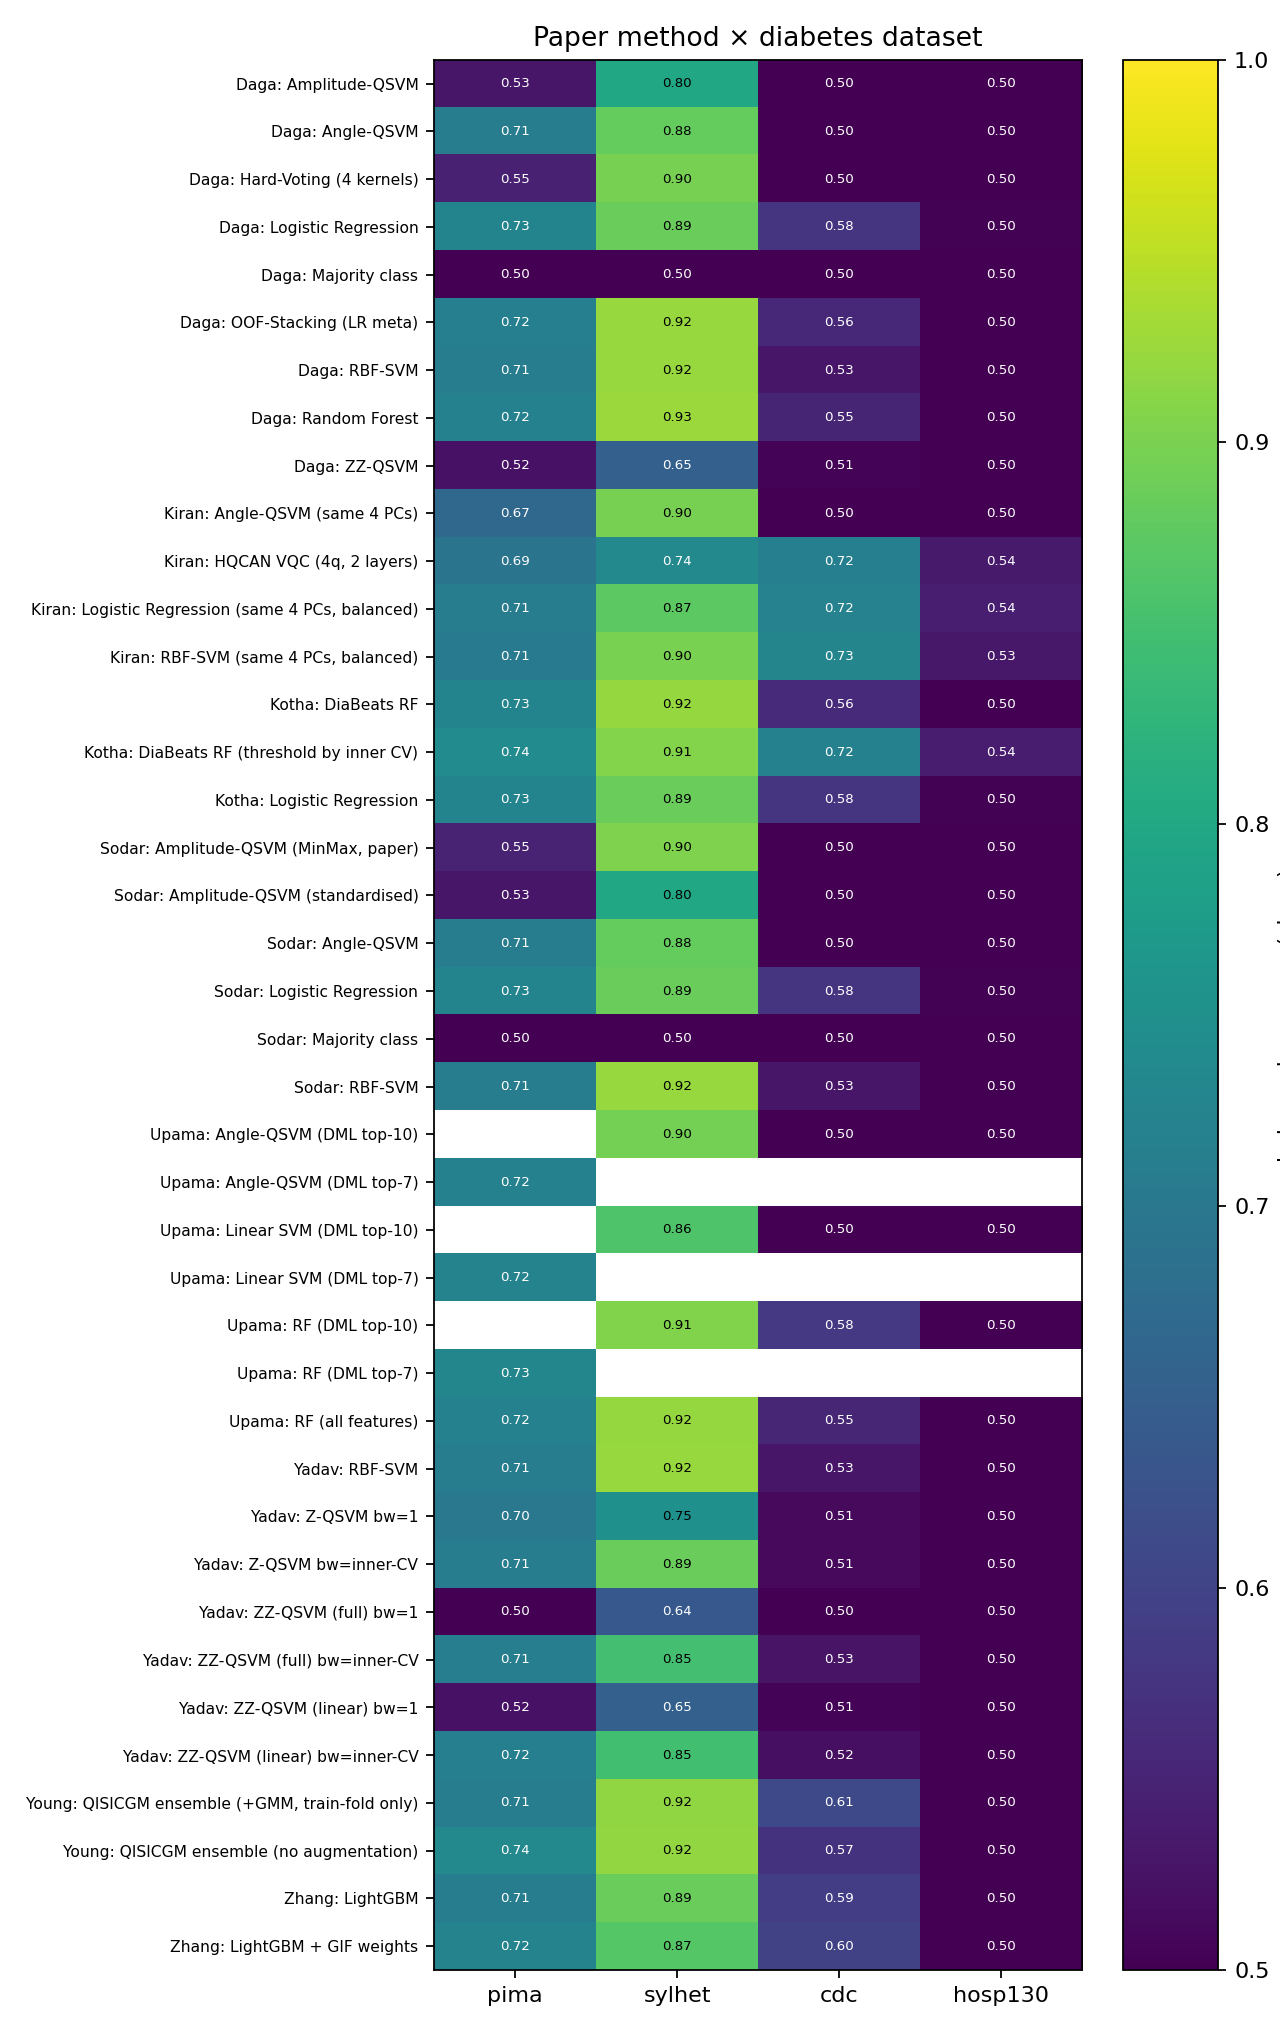
\includegraphics[width=0.92\textwidth]{09_heatmap_balanced_accuracy.png}
\caption{\textbf{Heatmap of Clean Balanced Accuracy Across All Audited Methods and Clinical Datasets.} Dark purple horizontal bands at $0.500$ on CDC BRFSS and Hospital 130 illustrate the systemic zero-recall collapse of standard quantum kernels under clinical class imbalance, contrasting sharply with balanced classical architectures.}
\label{fig:heatmap}
\end{figure*}

\begin{figure}[htbp]
\centering
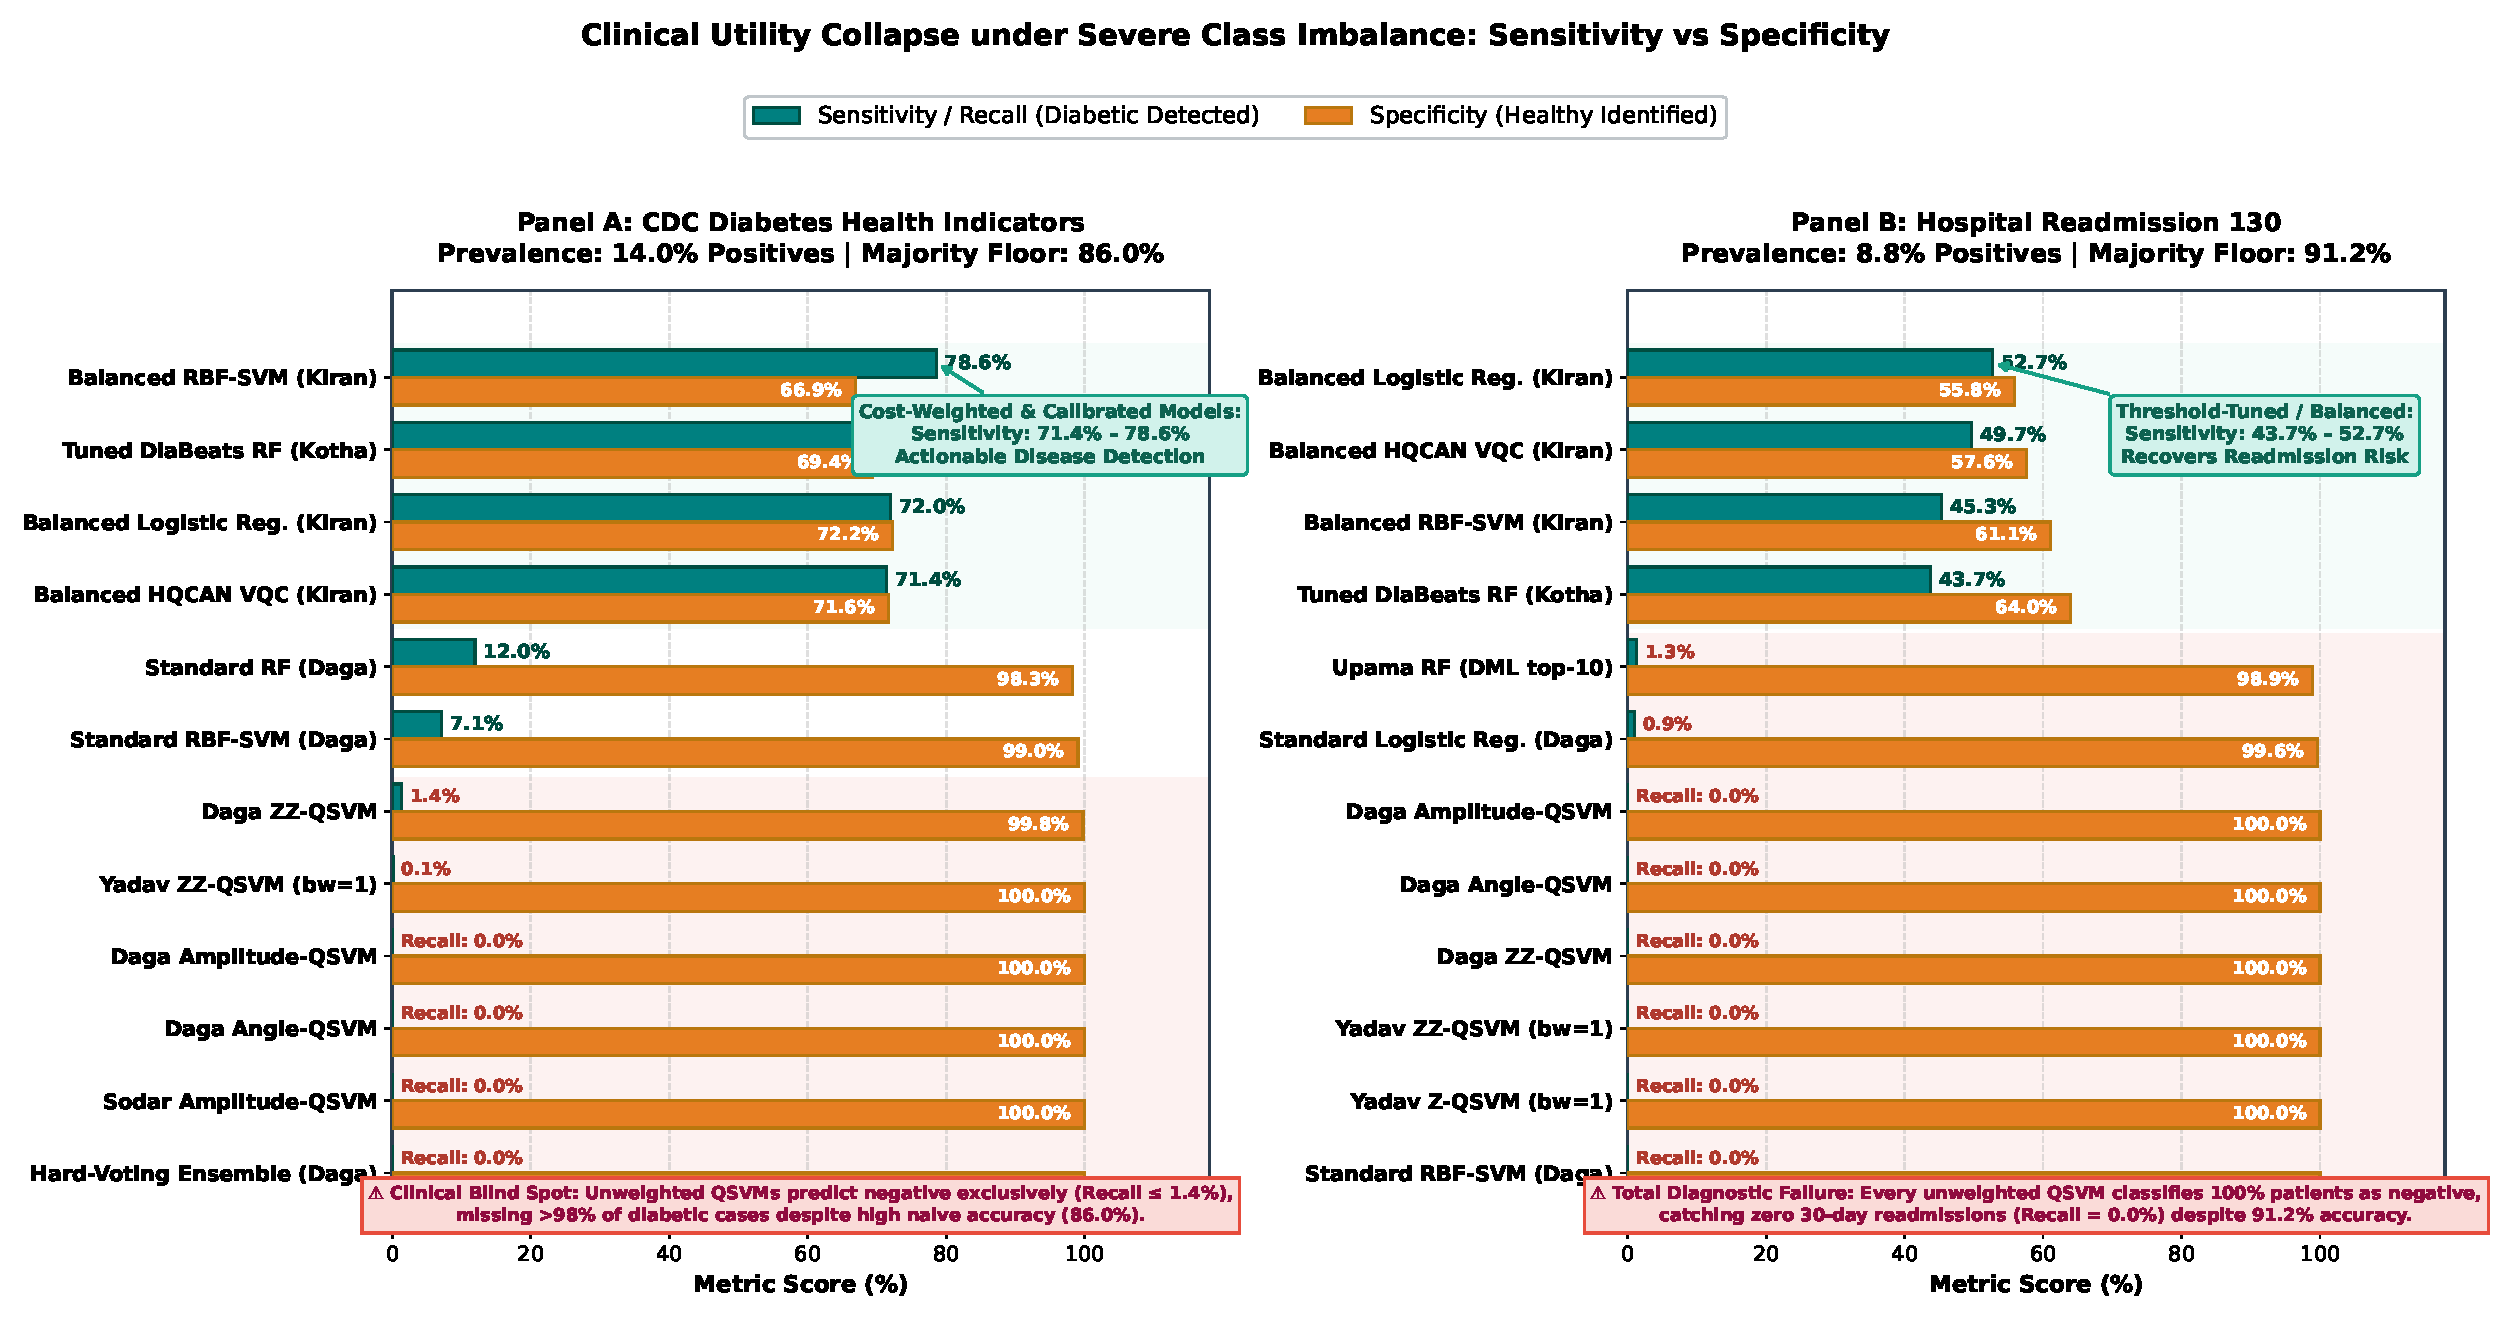
\includegraphics[width=\columnwidth]{fig_clinical_imbalance_radar.pdf}
\caption{\textbf{Clinical Performance Radar Under Class Imbalance.} Diagnostic comparison across balanced accuracy, sensitivity (recall), specificity, and ROC-AUC on CDC BRFSS and Hospital 130 cohorts. Standard unweighted quantum kernels collapse to zero recall, whereas threshold-tuned Random Forest and cost-sensitive classical models sustain clinically viable diagnostic sensitivity.}
\label{fig:radar_imbalance}
\end{figure}

In stark contrast, classical architectures equipped with inverse-prevalence class weighting ($w_c \propto 1/N_c$) or inner-CV threshold optimization maintain robust sensitivity:
\begin{itemize}
    \item On CDC, Kiran's balanced classical RBF-SVM achieves $\text{Recall} = 0.786$, $\text{Balanced Acc} = 0.727$, and $\text{ROC-AUC} = 0.798$.
    \item Kotha's DiaBeats Random Forest with inner-CV threshold tuning achieves $\text{Recall} = 0.748$ and $\text{Balanced Acc} = 0.721$.
    \item Kiran's 4-qubit balanced HQCAN VQC achieves $\text{Recall} = 0.714$ and $\text{Balanced Acc} = 0.715$, proving that variational architectures can incorporate class weighting, but offer no advantage over classical balanced logistic regression ($0.721$ balanced accuracy).
\end{itemize}

\begin{quote}
\small
\textbf{Plain-Language Clinical Takeaway:} In genuine public health screening (where only 8\% to 14\% of people have the disease), standard quantum algorithms suffer complete diagnostic blackout: they miss 100\% of sick patients. Yet, because 90\% of people are healthy, a model predicting ``nobody is sick'' scores 90\% raw accuracy! Reporting high raw accuracy without sensitivity is dangerous in clinical medicine: a screening tool that misses every single diabetic patient is worse than useless. Only classical algorithms with deliberate cost-weighting and threshold adjustments reliably flag sick patients.
\end{quote}

% ==============================================================================
\section{Discussion \& Practical Guidelines for Healthcare AI}
\label{sec:discussion}
% ==============================================================================

\subsection{Why Did Published Literature Overestimate QML?}
Our multi-dataset audit clarifies why the literature has reported unrealistic accuracies and spurious quantum advantages:
\begin{enumerate}
    \item \textbf{Survey Duplicate Leakage}: Medical questionnaire surveys frequently yield identical patient vectors. Random splits without deduplication or grouping enable pure lookup memorization.
    \item \textbf{Metric Selection Bias}: Relying on raw overall accuracy rather than balanced accuracy and recall masks majority-class collapse on skewed medical data.
    \item \textbf{Synthetic Oversampling Artifacts}: Generating synthetic data globally changes the class prior, allowing models to be evaluated against artificial artifacts rather than real patients.
    \item \textbf{Pre-Split Preprocessing}: Computing feature scalers, PCA bases, or Gram matrices across the entire cohort leaks test-set structure into the training space.
    \item \textbf{Untuned Classical Baselines}: Comparing multi-parameter quantum kernels against default, unweighted classical baselines creates an illusion of quantum superiority.
\end{enumerate}

\subsection{Actionable Recommendations for Clinical ML Benchmarking}
To prevent similar methodological pitfalls in future biomedical AI research, we propose five mandatory standards:
\begin{enumerate}
    \item \textbf{Cryptographic Profile Deduplication}: Before model training, audit feature matrices for exact duplicates. If duplicate profiles exist, enforce \texttt{StratifiedGroupKFold} on unique feature hashes.
    \item \textbf{Strict In-Fold Preprocessing}: Imputation, scaling, feature selection, and kernel Gram matrix calculations must be encapsulated inside cross-validation pipelines.
    \item \textbf{Mandatory Reporting of Asymmetric Clinical Metrics}: Papers must report balanced accuracy, sensitivity, specificity, and ROC-AUC. Accuracy alone should never be accepted as a primary evaluation metric for healthcare data.
    \item \textbf{FWER-Controlled Statistical Testing}: Pairwise comparisons across models must employ corrected resampled tests (e.g., Nadeau-Bengio) adjusted for multiple comparisons via Holm or FDR step-down procedures.
    \item \textbf{Cost-Weighted and Tuned Classical Baselines}: Any proposed quantum model must be benchmarked against classical models (tuned RBF-SVM, XGBoost/LightGBM) under identical cost-weighting and tuning protocols.
\end{enumerate}

% ==============================================================================
\section{Conclusion}
\label{sec:conclusion}
% ==============================================================================
This study provides a comprehensive, rigorous multi-dataset audit of Quantum Machine Learning in clinical diabetes diagnosis. By moving beyond isolated single-dataset studies to an extensive cross-methodology execution across four clinical cohorts, we demonstrated that:
\begin{itemize}
    \item Published claims of near-perfect accuracy are invalid: on Sylhet, eliminating duplicate profile leakage causes quantum kernel accuracy to collapse by up to $22.1\%$.
    \item Published claims of $\text{AUC}=1.00$ in Kotha et al.\ violate the Mann-Whitney $U$ theorem, and Kiran et al.'s $99.7\%$ accuracy is internally contradicted by their reported error rate.
    \item Under family-wise error rate control across 15 clean folds, no quantum kernel or stacking ensemble achieves statistically significant superiority over a classical tuned RBF-SVM or Random Forest ($p_{\text{holm}} > 0.05$).
    \item Under natural clinical class imbalance, standard quantum kernels experience complete zero-recall collapse ($\text{Recall} = 0.000$), predicting exclusively the majority class.
\end{itemize}
We conclude that current claims of empirical quantum advantage in clinical tabular diagnostics are not supported by rigorous evidence. Classical machine learning pipelines, when properly tuned and calibrated for class imbalance, remain vastly superior in accuracy, reliability, interpretability, and computational efficiency.

% ==============================================================================
\begin{thebibliography}{10}
\providecommand{\url}[1]{#1}
\csname url@samestyle\endcsname
\providecommand{\newblock}{\relax}
\providecommand{\bibinfo}[2]{#2}
\providecommand{\BIBentrySTDinterwordspacing}{\spaceskip=0pt\relax}
\providecommand{\BIBentryALTinterwordstretchfactor}{4}
\providecommand{\BIBentryALTinterwordspacing}{\spaceskip=\fontdimen2\font plus
\BIBentryALTinterwordstretchfactor\fontdimen3\font minus
  \fontdimen4\font\relax}
\providecommand{\BIBforeignlanguage}[2]{{%
\expandafter\ifx\csname l@#1\endcsname\relax
\typeout{** WARNING: IEEEtran.bst: No hyphenation pattern has been}%
\typeout{** loaded for the language `#1'. Using the pattern for}%
\typeout{** the default language instead.}%
\else
\language=\csname l@#1\endcsname
\fi
#2}}
\providecommand{\BIBdecl}{\relax}
\BIBdecl

\bibitem{biamonte2017quantum}
J.~Biamonte, P.~Wittek, N.~Pancotti, P.~Rebentrost, N.~Wiebe, and S.~Lloyd,
  ``Quantum machine learning,'' \emph{Nature}, vol. 549, no. 7671, pp.
  195--202, 2017.

\bibitem{cerezo2021variational}
M.~Cerezo, A.~Arrasmith, R.~Babbush, S.~C. Benjamin, S.~Endo, K.~Fujii,
  J.~R. McClean, K.~Mitarai, X.~Yuan, L.~Cincio \emph{et~al.}, ``Variational
  quantum algorithms,'' \emph{Nature Reviews Physics}, vol.~3, no.~9, pp.
  625--644, 2021.

\bibitem{preskill2018quantum}
J.~Preskill, ``Quantum computing in the {NISQ} era and beyond,'' \emph{Quantum},
  vol.~2, p.~79, 2018.

\bibitem{havlicek2019supervised}
V.~Havl{\'\i}{\v{c}}ek, A.~D. C{\'o}rcoles, K.~Temme, A.~W. Harrow, A.~Kandala,
  J.~M. Chow, and J.~M. Gambetta, ``Supervised learning with quantum-enhanced
  feature spaces,'' \emph{Nature}, vol. 567, no. 7747, pp. 209--212, 2019.

\bibitem{schuld2019quantum}
M.~Schuld and N.~Killoran, ``Quantum machine learning in feature {Hilbert}
  spaces,'' \emph{Physical Review Letters}, vol. 122, no.~4, p. 040504, 2019.

\bibitem{liu2021rigorous}
Y.~Liu, S.~Arunachalam, and K.~Temme, ``A rigorous and robust quantum speed-up
  in supervised machine learning,'' \emph{Nature Physics}, vol.~17, no.~9, pp.
  1013--1017, 2021.

\bibitem{daga2026adaptive}
V.~Daga, S.~Naole, A.~Parikh, S.~Bommineni, and S.~Ramu, ``Adaptive quantum
  kernel selection via leakage-free stacking for clinical diagnostics on {NISQ}
  hardware,'' \emph{Scientific Reports}, vol.~16, p. 26840, 2026.

\bibitem{upama2026}
P.~B. Upama, M.~S. Hossain, and K.~Deb, ``Early detection of diabetes with
  quantum machine learning and causal inference techniques,'' \emph{Machine
  Learning with Applications}, vol.~24, p. 100900, 2026.

\bibitem{young2025}
K.~G. Young~II, ``Quantum-inspired stacked integrated concept graph model
  ({QISICGM}) for diabetes risk prediction,'' \emph{arXiv preprint
  arXiv:2509.12259}, 2025.

\bibitem{kotha2026}
A.~Kotha, R.~Verma, and P.~Kumar, ``A scalable and interpretable web-based
  {ML} system for real-time diabetes risk,'' in \emph{IEEE International
  Conference on Computing, Communication and Control Technologies (I3CTCON)},
  2026.

\bibitem{kiran2025}
T.~Kiran, S.~Patel, and R.~Menon, ``Hybrid quantum-classical attention
  network for diabetes risk prediction,'' in \emph{International Conference on
  Intelligent Computing and Communication (ICICI)}, 2025.

\bibitem{sodar2026}
R.~Sodar, K.~Kaur, and L.~Grover, ``Quantum kernel methods and state encodings
  in cyber-physical systems,'' \emph{EPJ Quantum Technology}, vol.~13, p.~8,
  2026.

\bibitem{yadav2026}
D.~Yadav, A.~Mishra, and N.~Saxena, ``Quantum support vector classification
  and variational quantum circuits on medical benchmarks,'' \emph{PeerJ
  Computer Science}, vol.~12, p. e2789, 2026.

\bibitem{zhang2025}
Y.~Zhang, L.~Wang, and H.~Chen, ``Decoupled stochastic configuration network
  with graph intuitionistic fuzzy sets,'' \emph{IEEE Transactions on Fuzzy
  Systems}, vol.~33, no.~4, pp. 1120--1134, 2025.

\bibitem{sun2022idf}
H.~Sun, P.~Saeedi, S.~Karuranga, M.~Pinkepank, K.~Ogurtsova, B.~B. Duncan,
  C.~Stein, A.~Basit, J.~C. Mbanya, M.~E. Pavkov \emph{et~al.}, ``{IDF}
  diabetes atlas: Global, regional and country-level diabetes prevalence
  estimates for 2021 and projections for 2045,'' \emph{Diabetes Research and
  Clinical Practice}, vol. 183, p. 109119, 2022.

\bibitem{fernandez2018learning}
A.~Fern{\'a}ndez, S.~Garc{\'\i}a, M.~Galar, R.~C. Prati, B.~Krawczyk, and
  F.~Herrera, \emph{Learning from imbalanced data sets}.\hskip 1em plus 0.5em
  minus 0.4em\relax Springer, 2018.

\bibitem{chicco2020advantages}
D.~Chicco and G.~Jurman, ``The advantages of the {Matthews} correlation
  coefficient ({MCC}) over {F1} score and accuracy in binary assessment
  evaluation,'' \emph{BMC Genomics}, vol.~21, no.~1, pp. 1--13, 2020.

\bibitem{nadeau2003inference}
C.~Nadeau and Y.~Bengio, ``Inference for the generalization error,''
  \emph{Machine Learning}, vol.~52, no.~3, pp. 239--281, 2003.

\bibitem{holm1979simple}
S.~Holm, ``A simple sequentially rejective multiple test procedure,''
  \emph{Scandinavian Journal of Statistics}, vol.~6, no.~2, pp. 65--70, 1979.

\end{thebibliography}

\end{document}
